\chapterx{Appendix B. Case Studies}
\sffamily\small
In the following sections we present three cases in which ccplot was used to produce plots of MODIS swath, CloudSat profile,
and CALIPSO profile and layer products. A brief analysis is provided with each case.

\section*{Case 1: Sand over Sahara, 28 June 2006}
This case was chosen to demonstrate typical appearance of sand suspended in the lower troposphere in CALIPSO profiles.
\vspace{3mm}

\noindent
\begin{minipage}[t]{60mm}
\textbf{a}, presented is a track over an area called Murzuq Desert in the south west of Libya between \ang{22}\,N and \ang{27}\,N. 
\textbf{b}, a layer of sand stretches predominantly from the ground to \SI{4}{km}. A conspicuous change in response occurs at \SI{8.1}{km}. This is due to change in sampling resolution between Region\,2 and Region\,3 as explained in Fig.\,\ref{fig:caliop-regions}. The thick band of high backscatter below the ground (red line) is caused by oversaturation of detectors, as can be seen in most \SI{532}{nm} profiles.
\end{minipage}\hfill
\begin{minipage}[t]{86mm}
\textsf{\small a)}\\
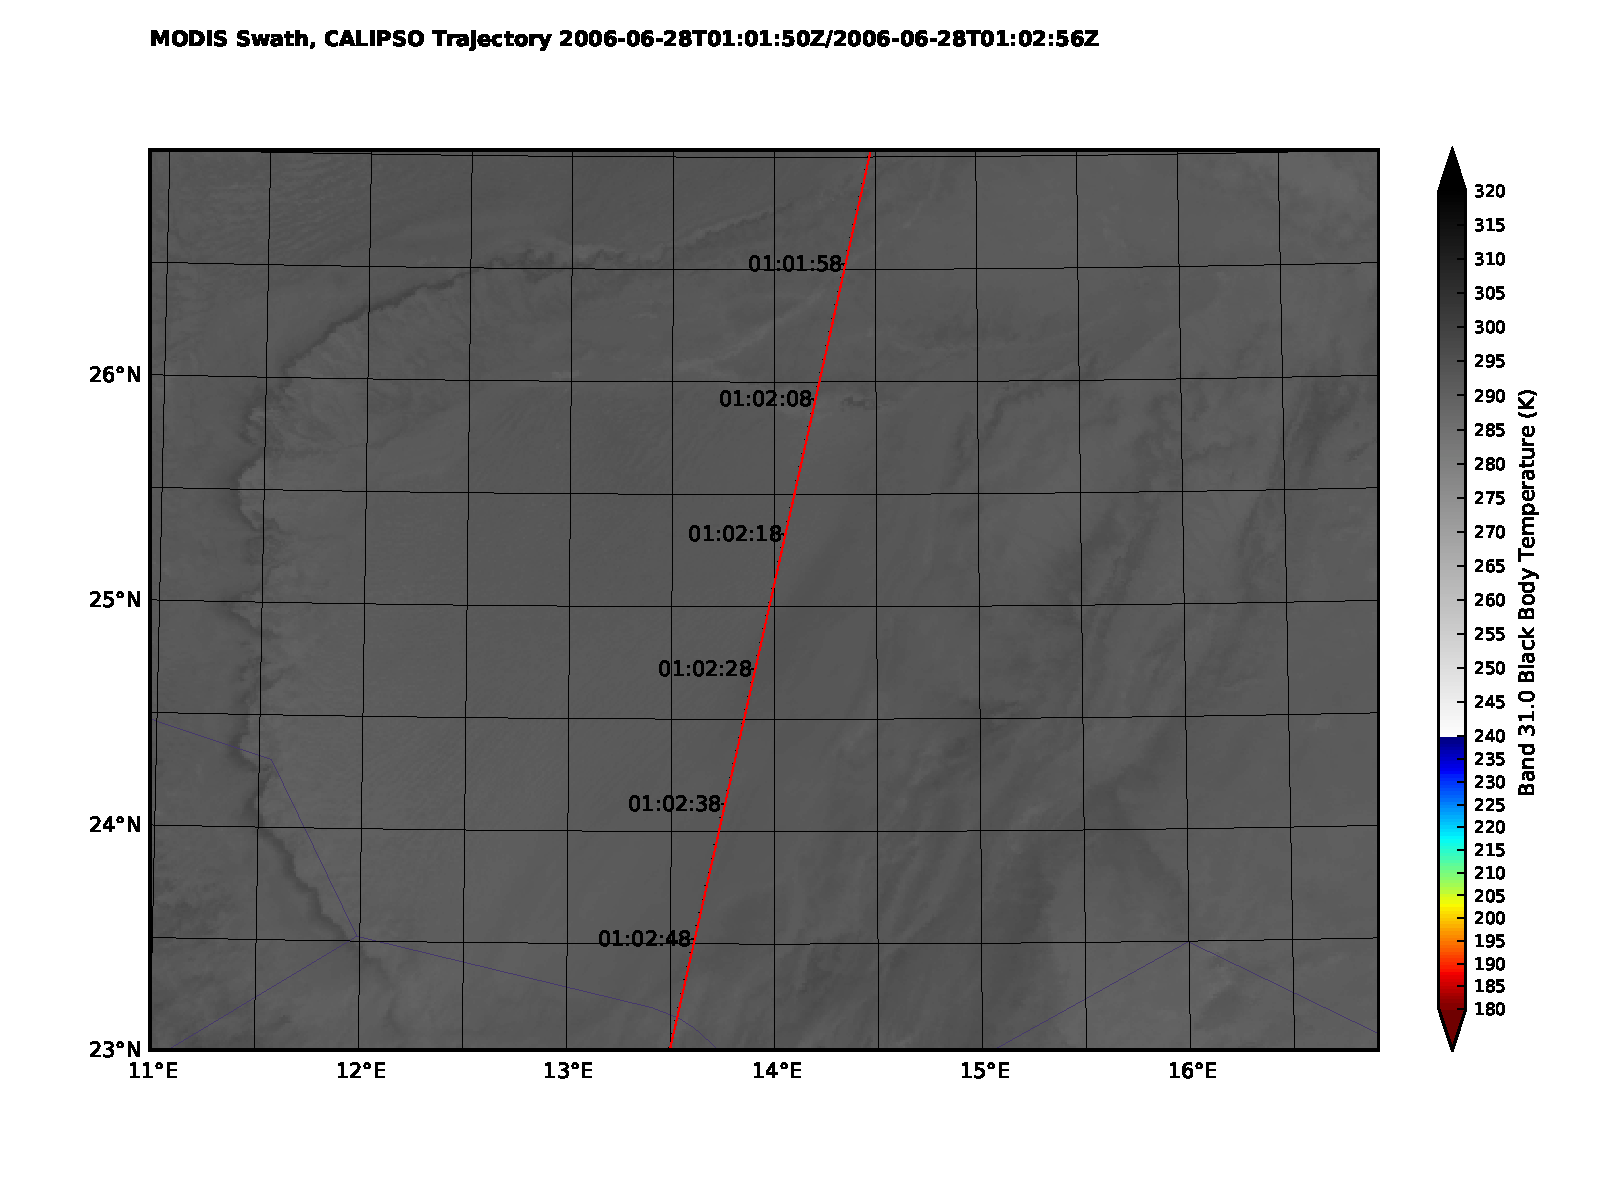
\includegraphics[width=86mm,clip,trim=10mm 10mm 4mm 4mm]{images/sahara/orbit-modis_x31+calipso.pdf}\\
\end{minipage}
\vspace{3mm}

\noindent\textsf{\small b)}\\
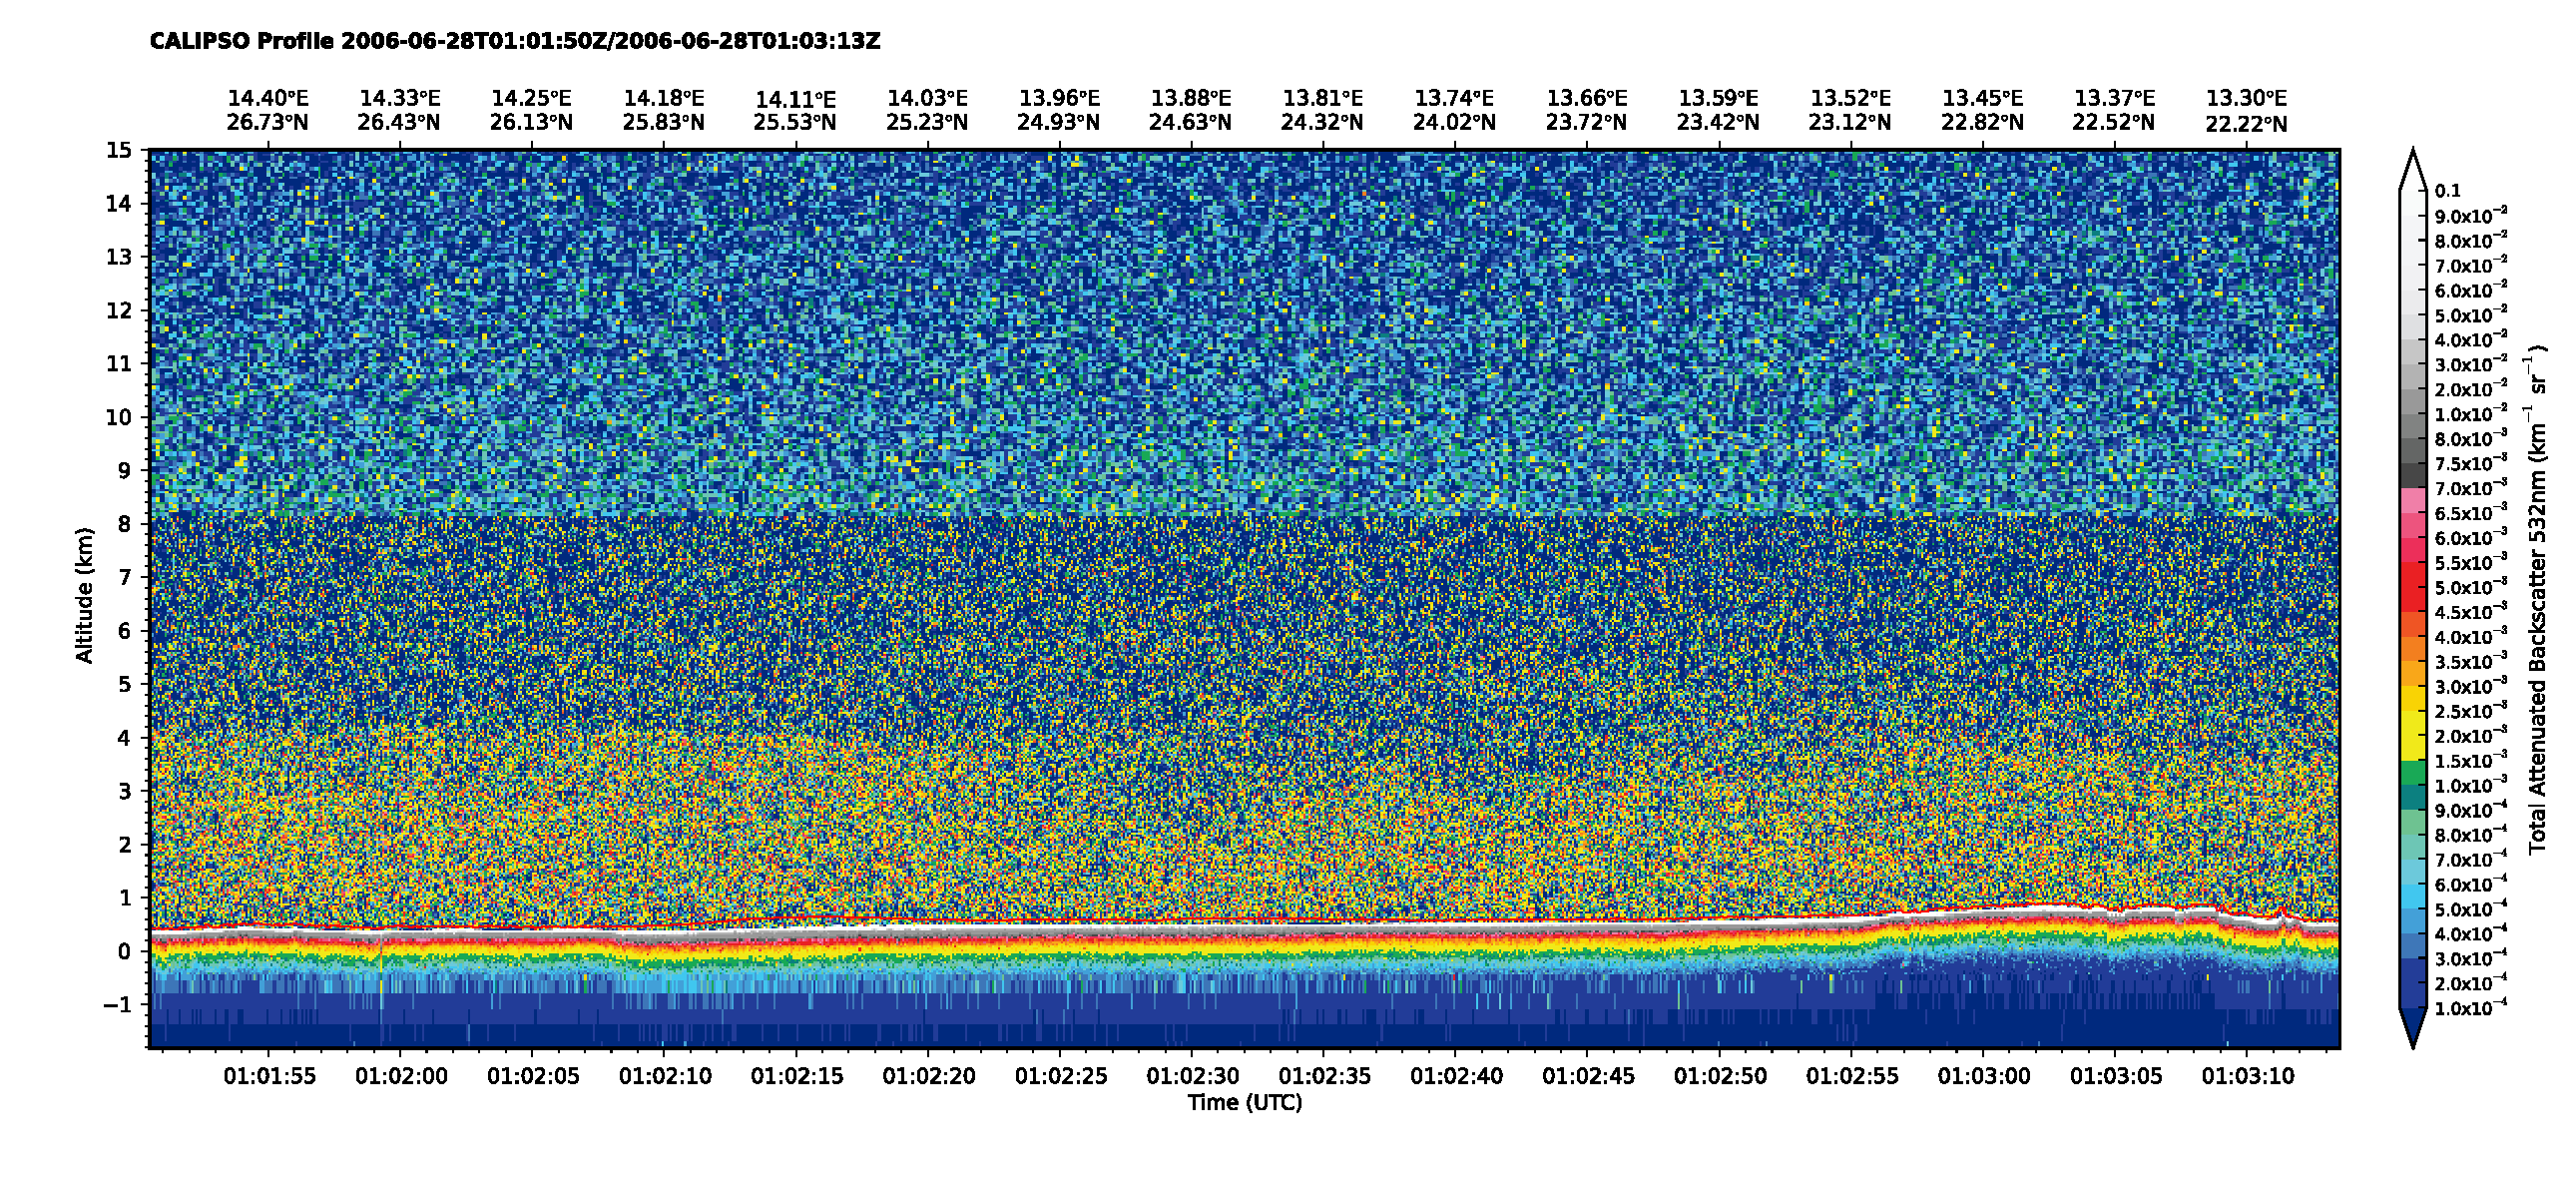
\includegraphics[width=150mm,clip,trim=10mm 10mm 4mm 4mm]{images/sahara/1calipso532.pdf}

\clearpage
\noindent
\textbf{c}, because sand particles are weak light polarisers, the response on Perpendicular Attenuated Backscatter \SI{532}{nm} is scattered and low.
\textbf{d}, response at \SI{1064}{nm} is slightly lower than at \SI{532}{nm}.
\vspace{3mm}

\noindent\textsf{\small c)}\\
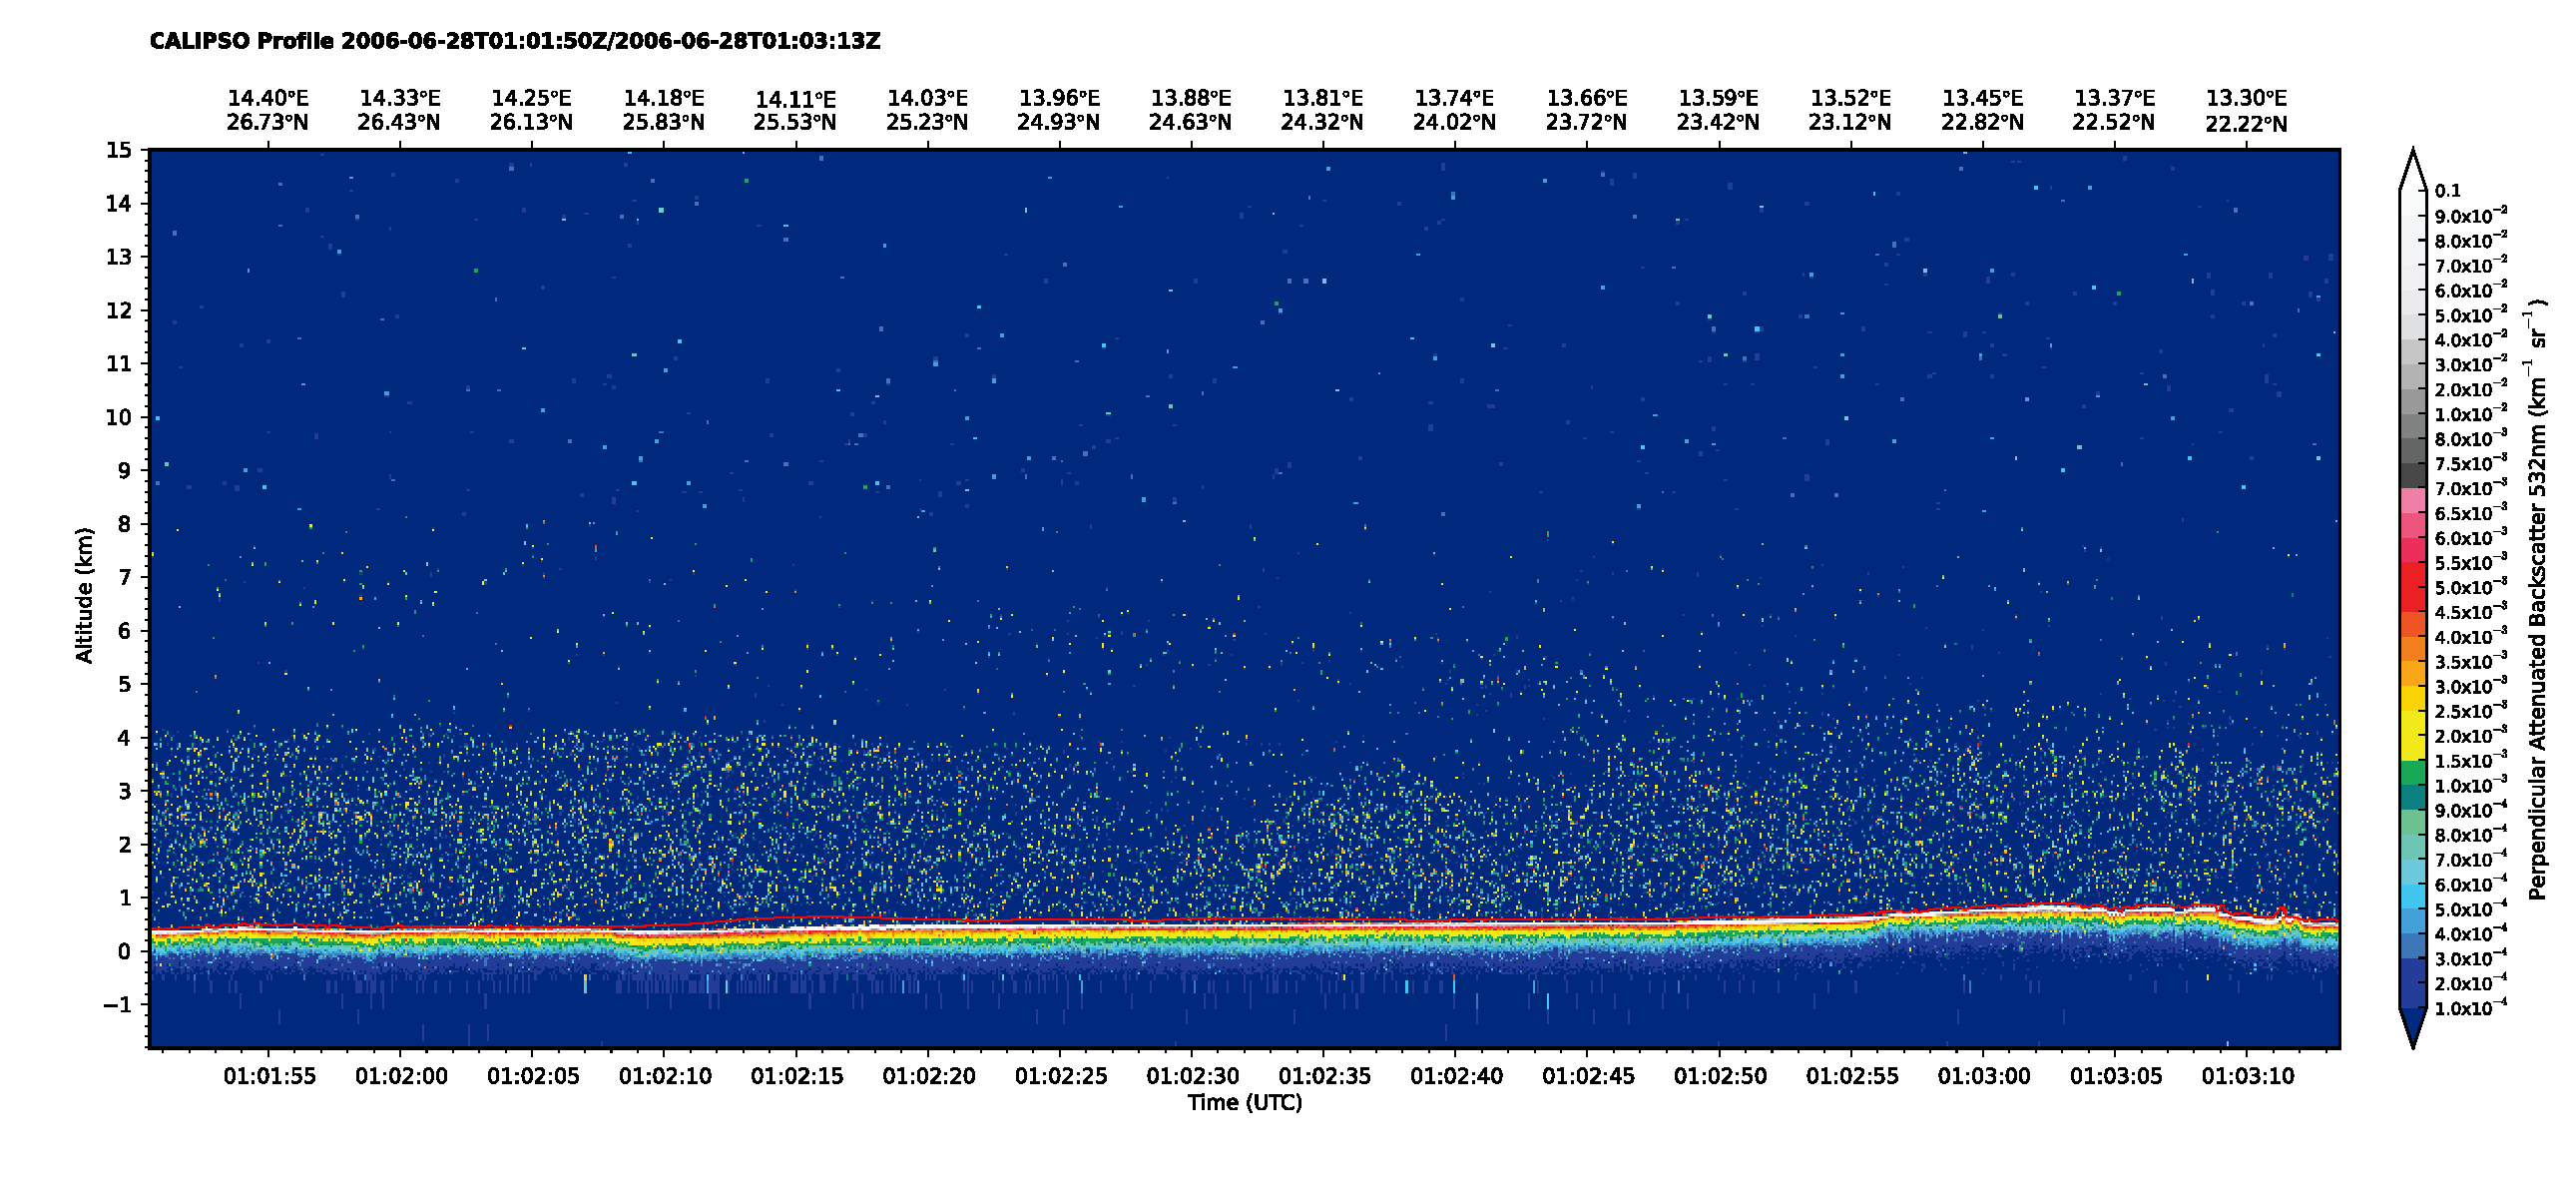
\includegraphics[width=150mm,clip,trim=10mm 10mm 4mm 4mm]{images/sahara/1calipso532p.pdf}\\
\noindent\textsf{\small d)}\\
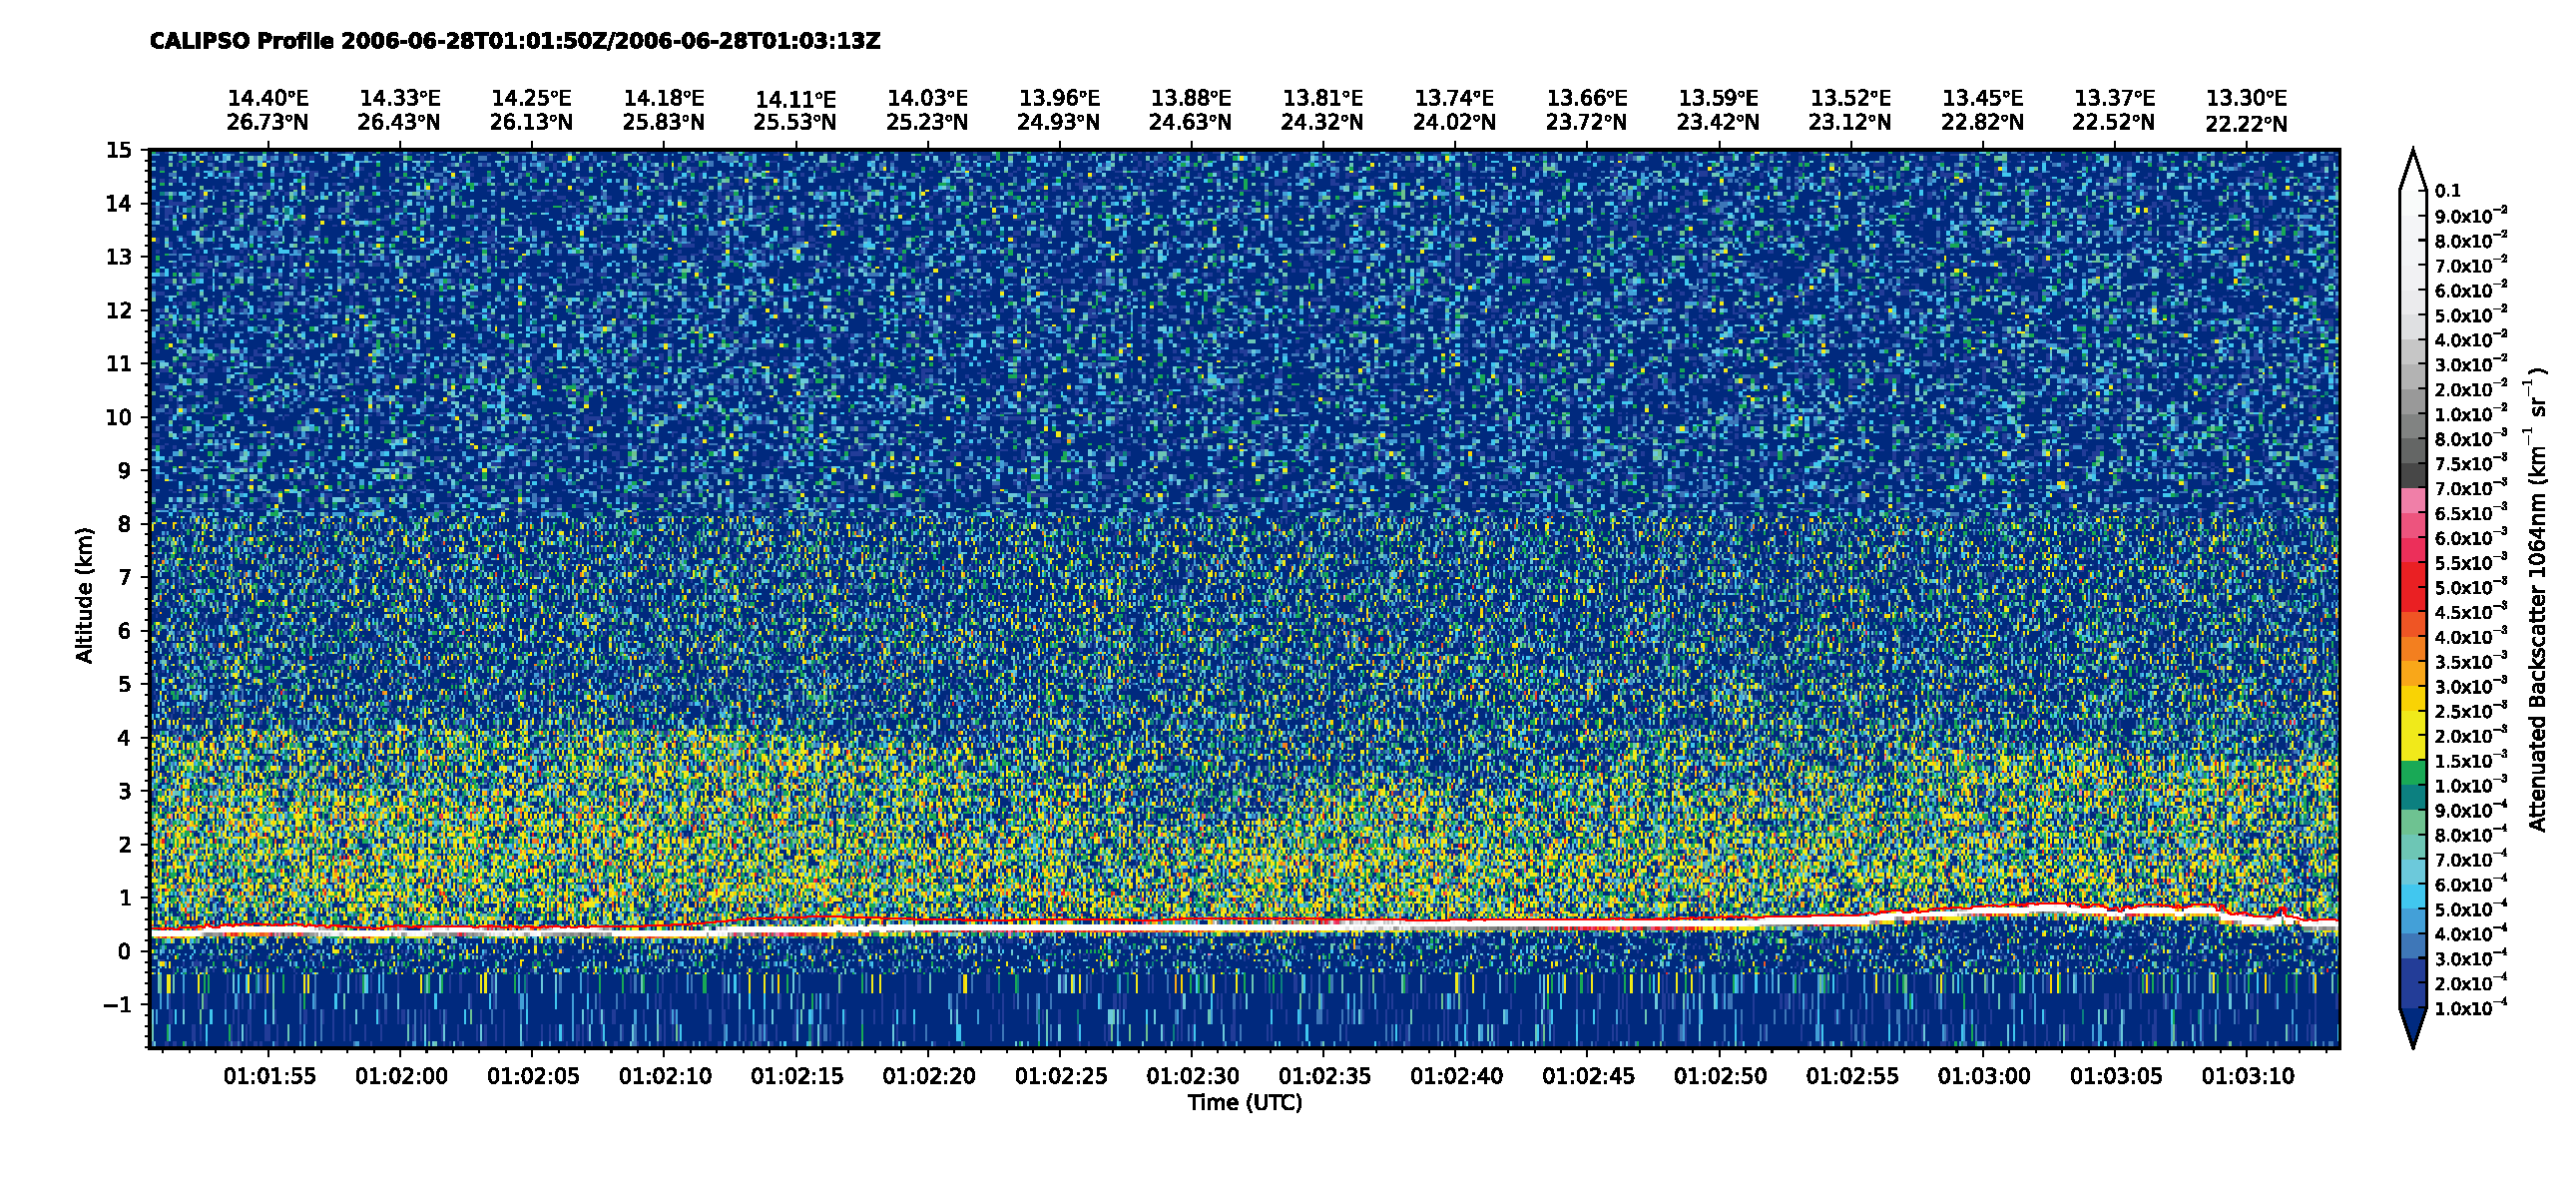
\includegraphics[width=150mm,clip,trim=10mm 10mm 4mm 4mm]{images/sahara/1calipso1064.pdf}

\clearpage
\section*{Case 2: Polar Stratospheric Clouds, Antarctica, 12 June 2007}
In this case we examine clouds inside the Antarctic Polar Vortex during the austral winter.
These conditions favour formation of Polar Stratospheric Clouds (PSCs),
which are crucial in converting reservoir species of chlorine into more active species,
leading to strong ozone depletion when sun rises in the austral spring.
\vspace{3mm}

\noindent
\begin{minipage}[t]{72mm}
\textbf{a}, this case presents a track over Palmer Land at the base of
Antarctic Peninsula between \ang{68}\,S and \ang{81}\,S, and \ang{58}\,W and \ang{102}\,W.
\textbf{b}, visible are two clouds, the larger one stretches up to
about \SI{13}{km}. It has a bottom part that touches the ground, but it is only
visible in the CloudSat profile, either because the
attenuation by the overlying layers is too high, or
because the bottom part is composed of larger particles
such as snow pellets. A much more faint second cloud is
visible at \SI{20}{km}.
\textbf{c}, light scattered from both clouds is polarised,
which indicates ice-phase clouds, as we would expect in
Antarctica in winter.
\end{minipage}\hfill
\begin{minipage}[t]{74mm}
\noindent\textsf{\small a)}\\
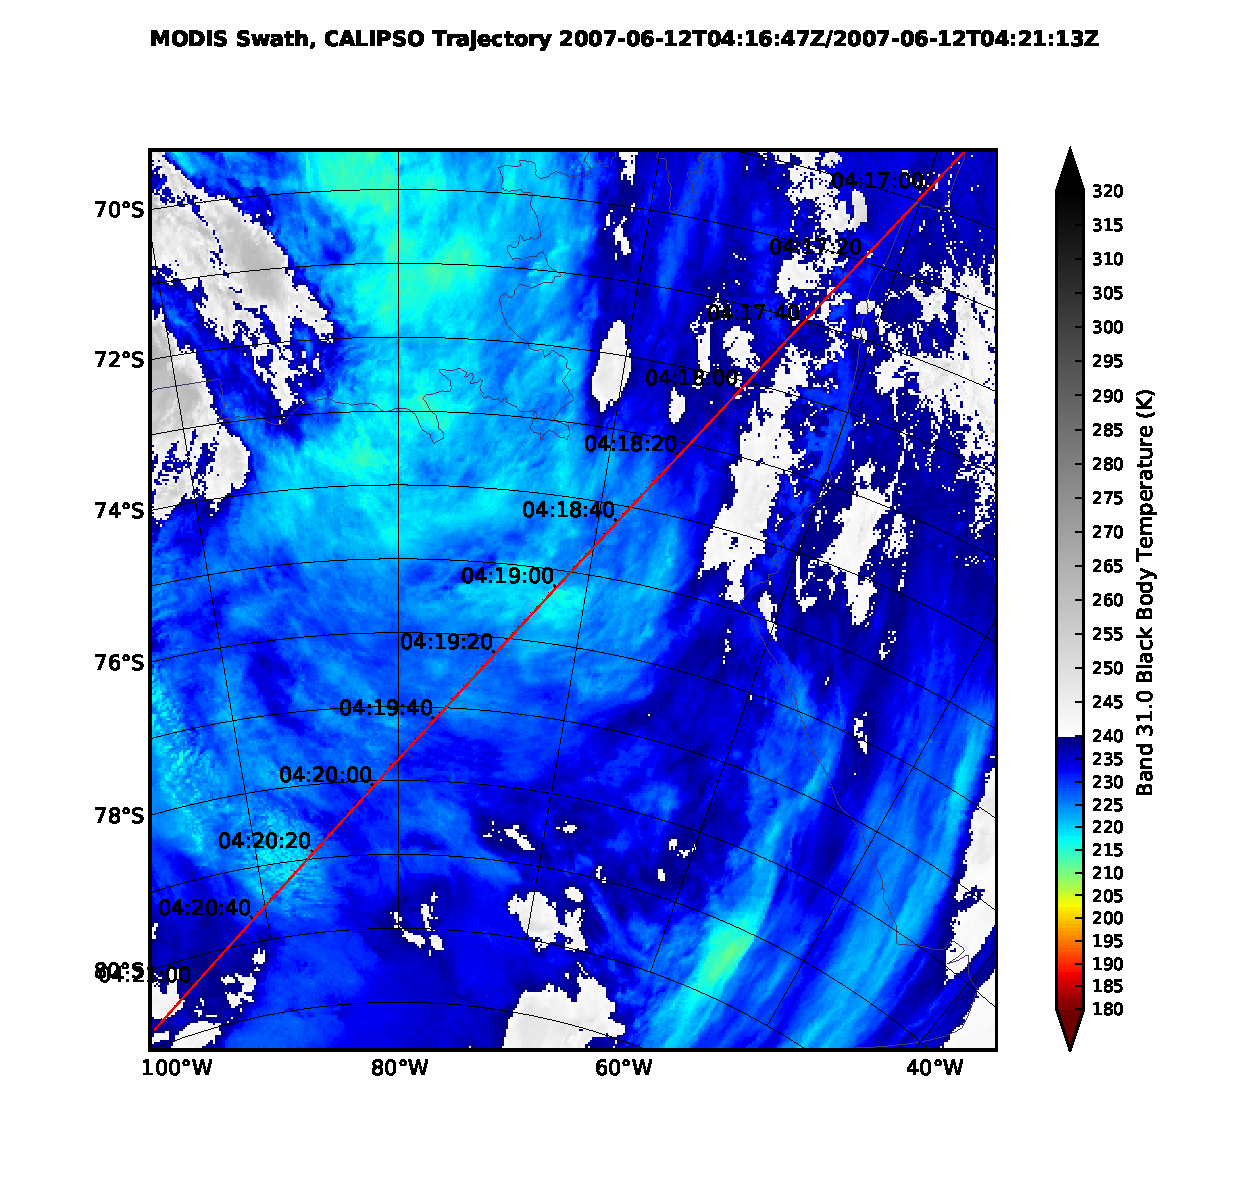
\includegraphics[width=74mm,clip,trim=10mm 10mm 4mm 4mm]{images/antarctica/orbit-modis_x31+calipso.pdf}
\end{minipage}

\noindent\textsf{\small b)}\\
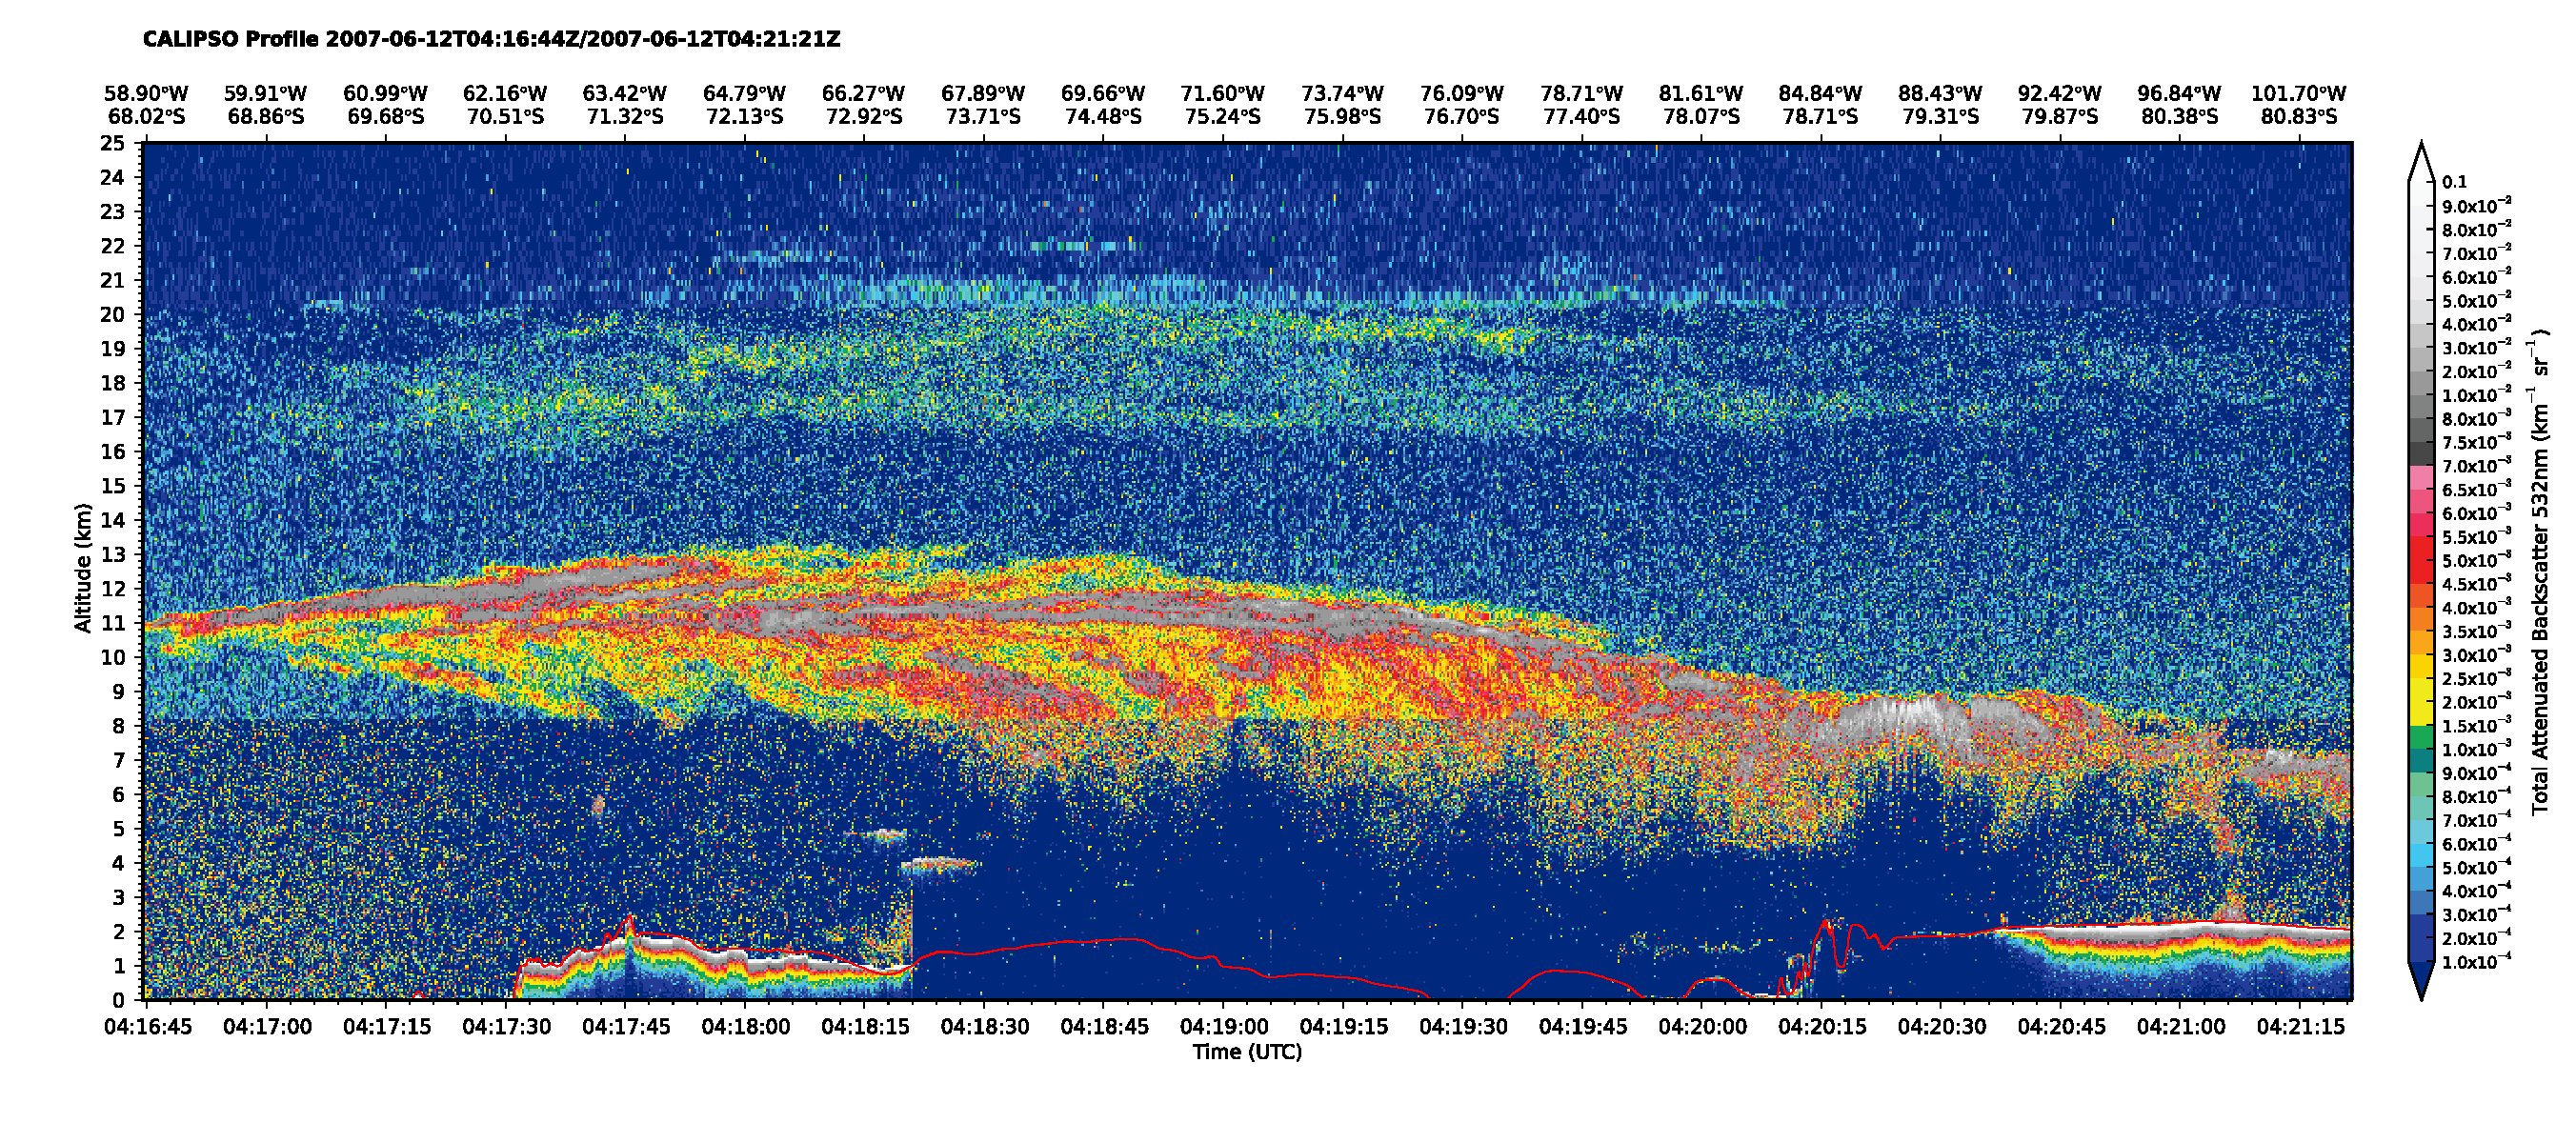
\includegraphics[width=140mm,clip,trim=10mm 10mm 4mm 4mm]{images/antarctica/1calipso532.pdf}\\
\noindent\textsf{\small c)}\\
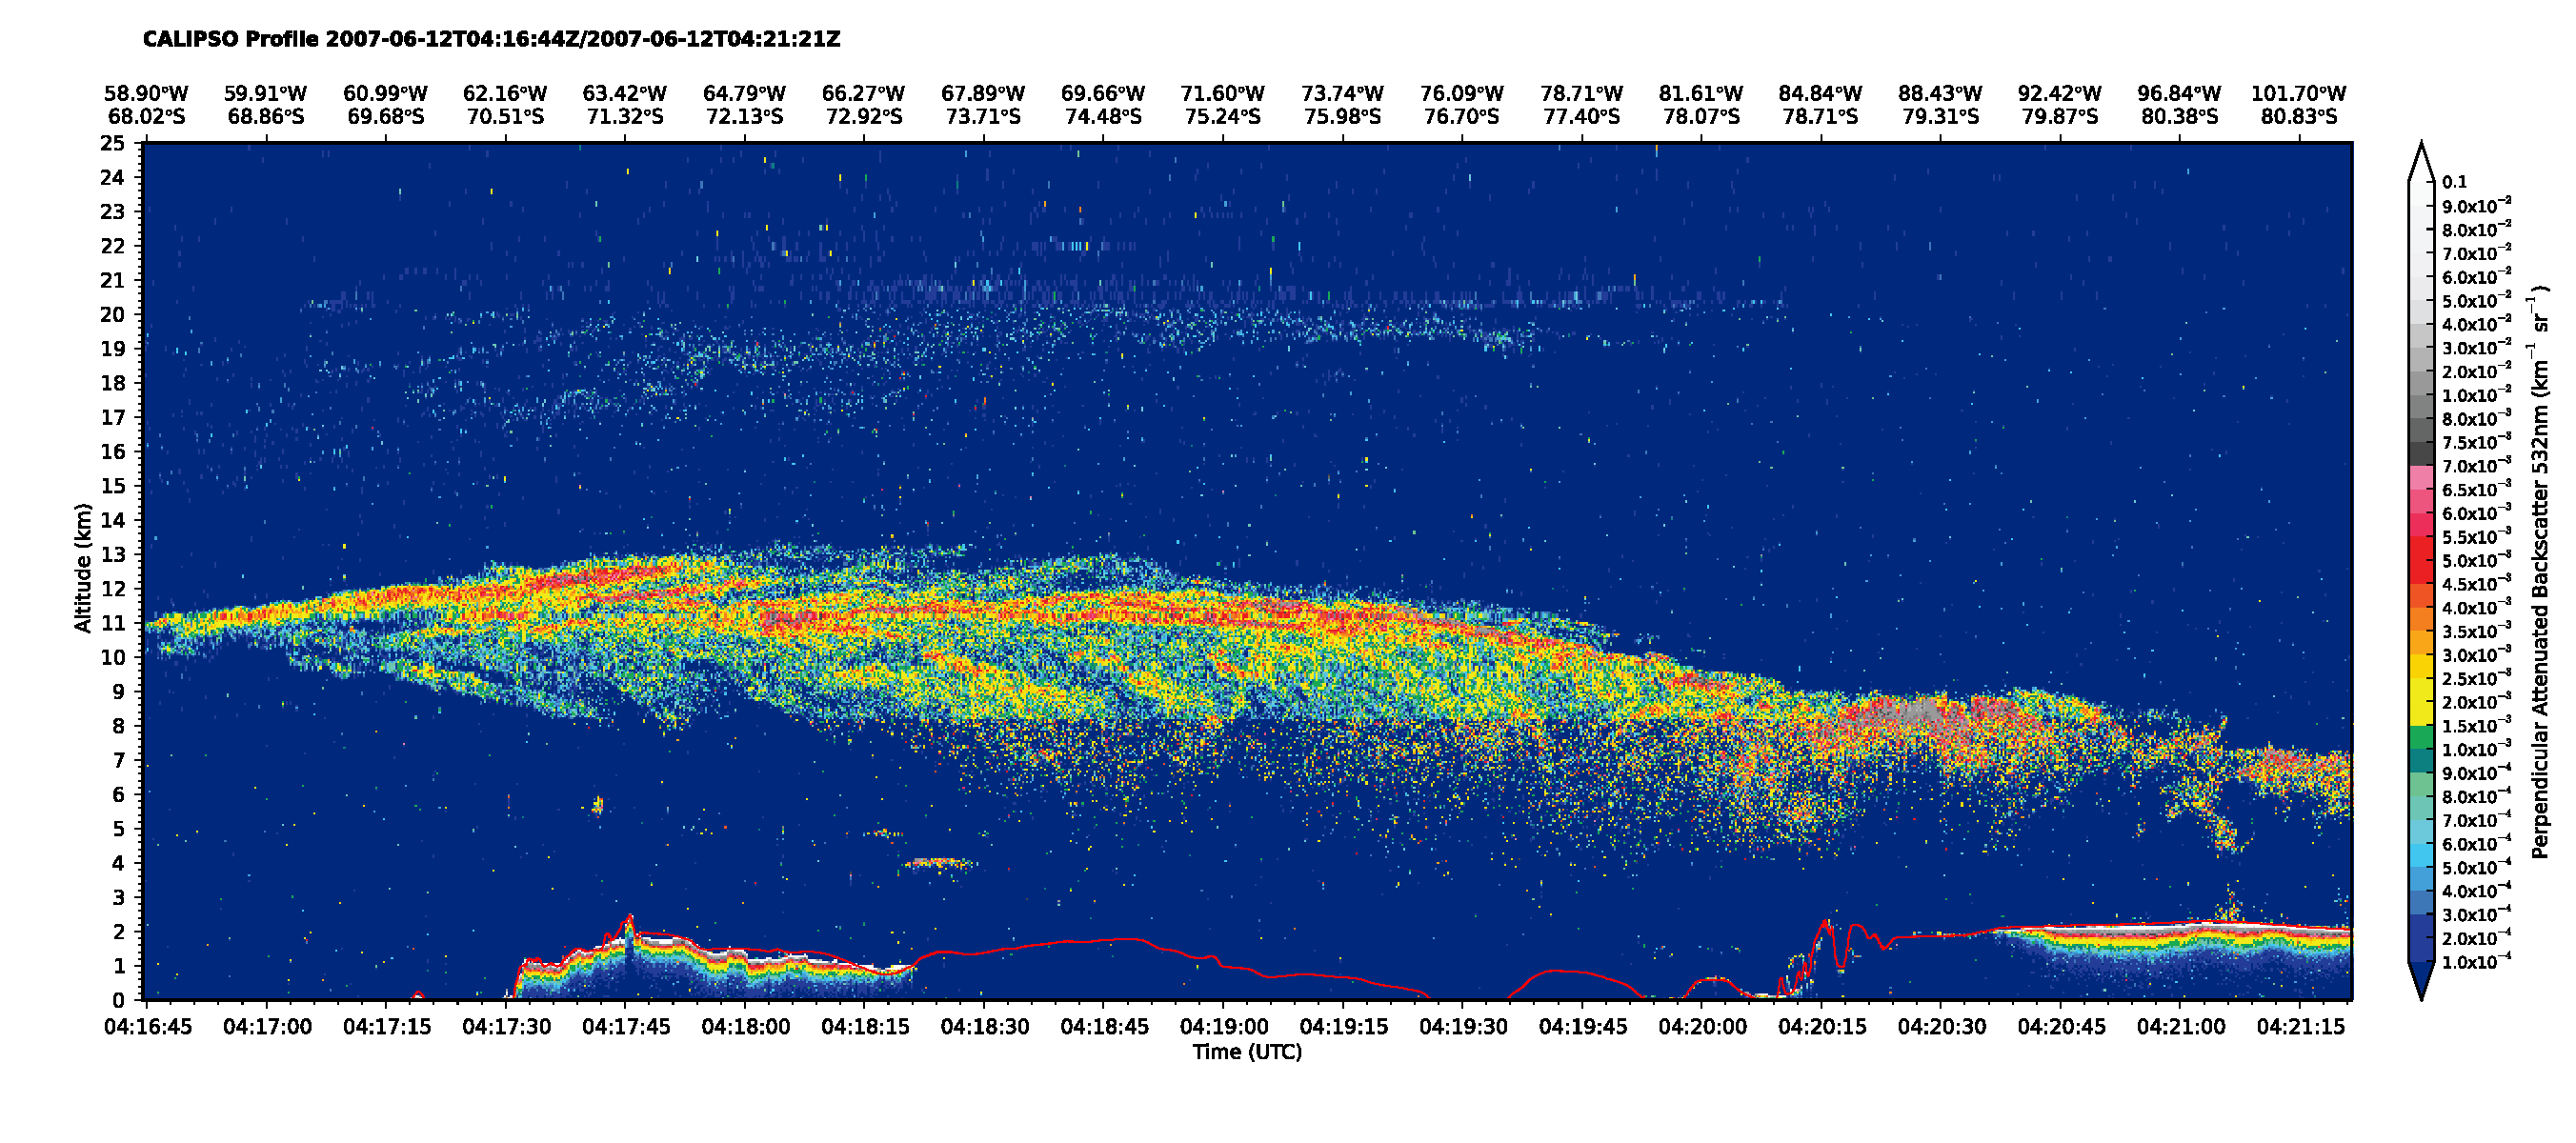
\includegraphics[width=140mm,clip,trim=10mm 10mm 4mm 4mm]{images/antarctica/1calipso532p.pdf}

\clearpage
\noindent
\textbf{d}, midlayer temperature of the lower cloud is greater than \SI{-78}{\celsius}, which is not enough
for PSCs to form, although the fainter cloud visible in profile products could be a PSC. \textbf{e}, the larger cloud was well recognised by the layer detection algorithm.
\vspace{3mm}

\noindent\textsf{\small d)}\\
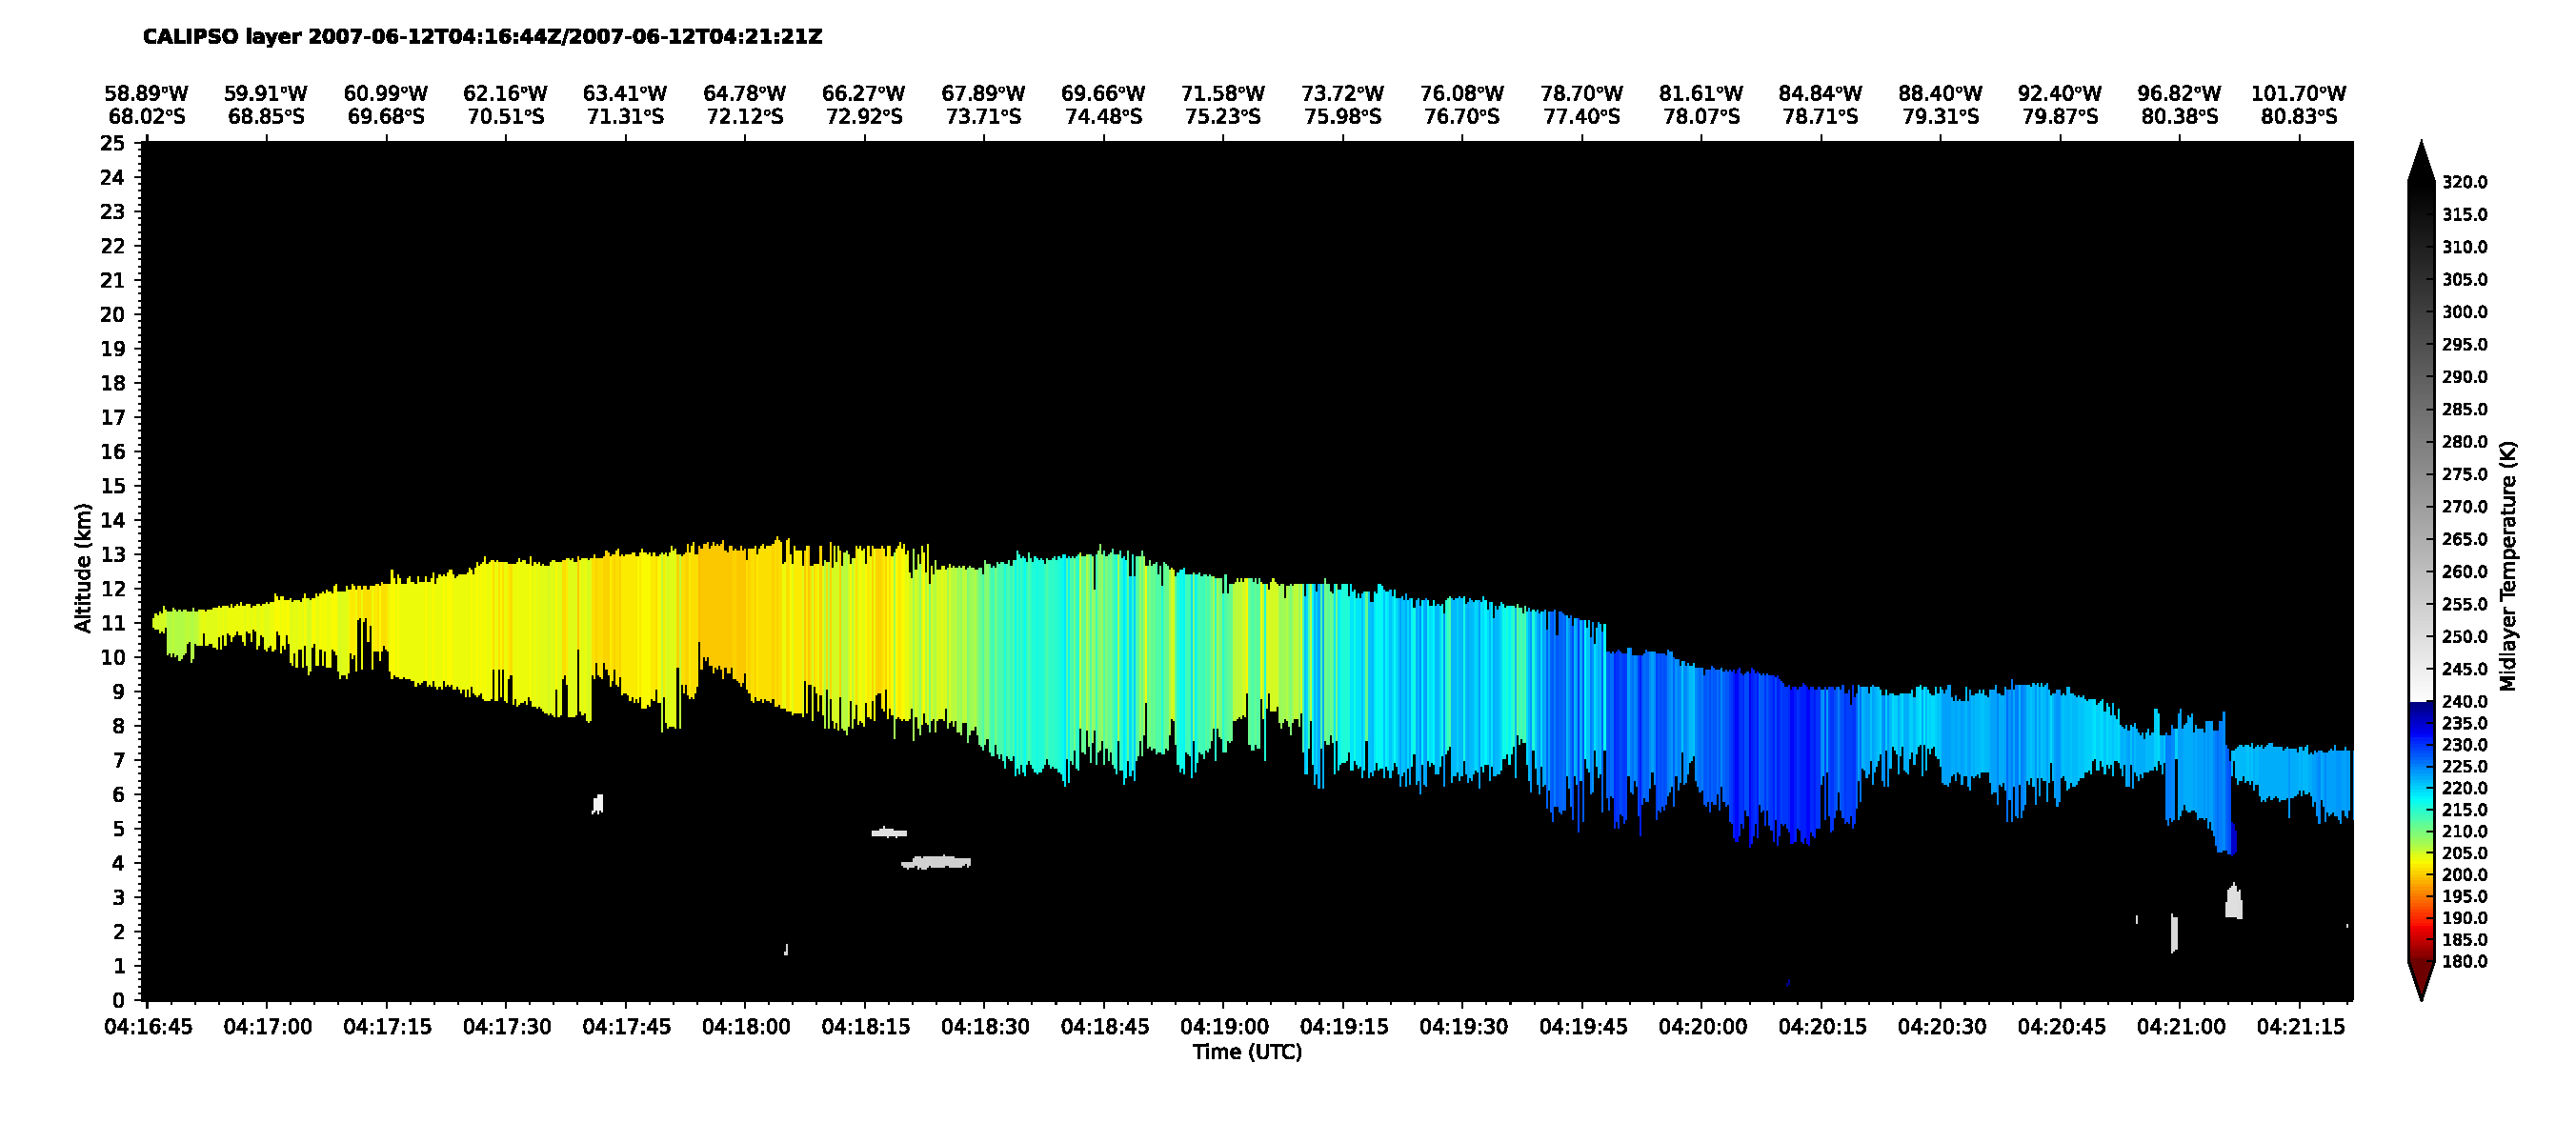
\includegraphics[width=150mm,clip,trim=10mm 10mm 4mm 4mm]{images/antarctica/1calipso-temperature-layer.pdf}\\
\noindent\textsf{\small e)}\\
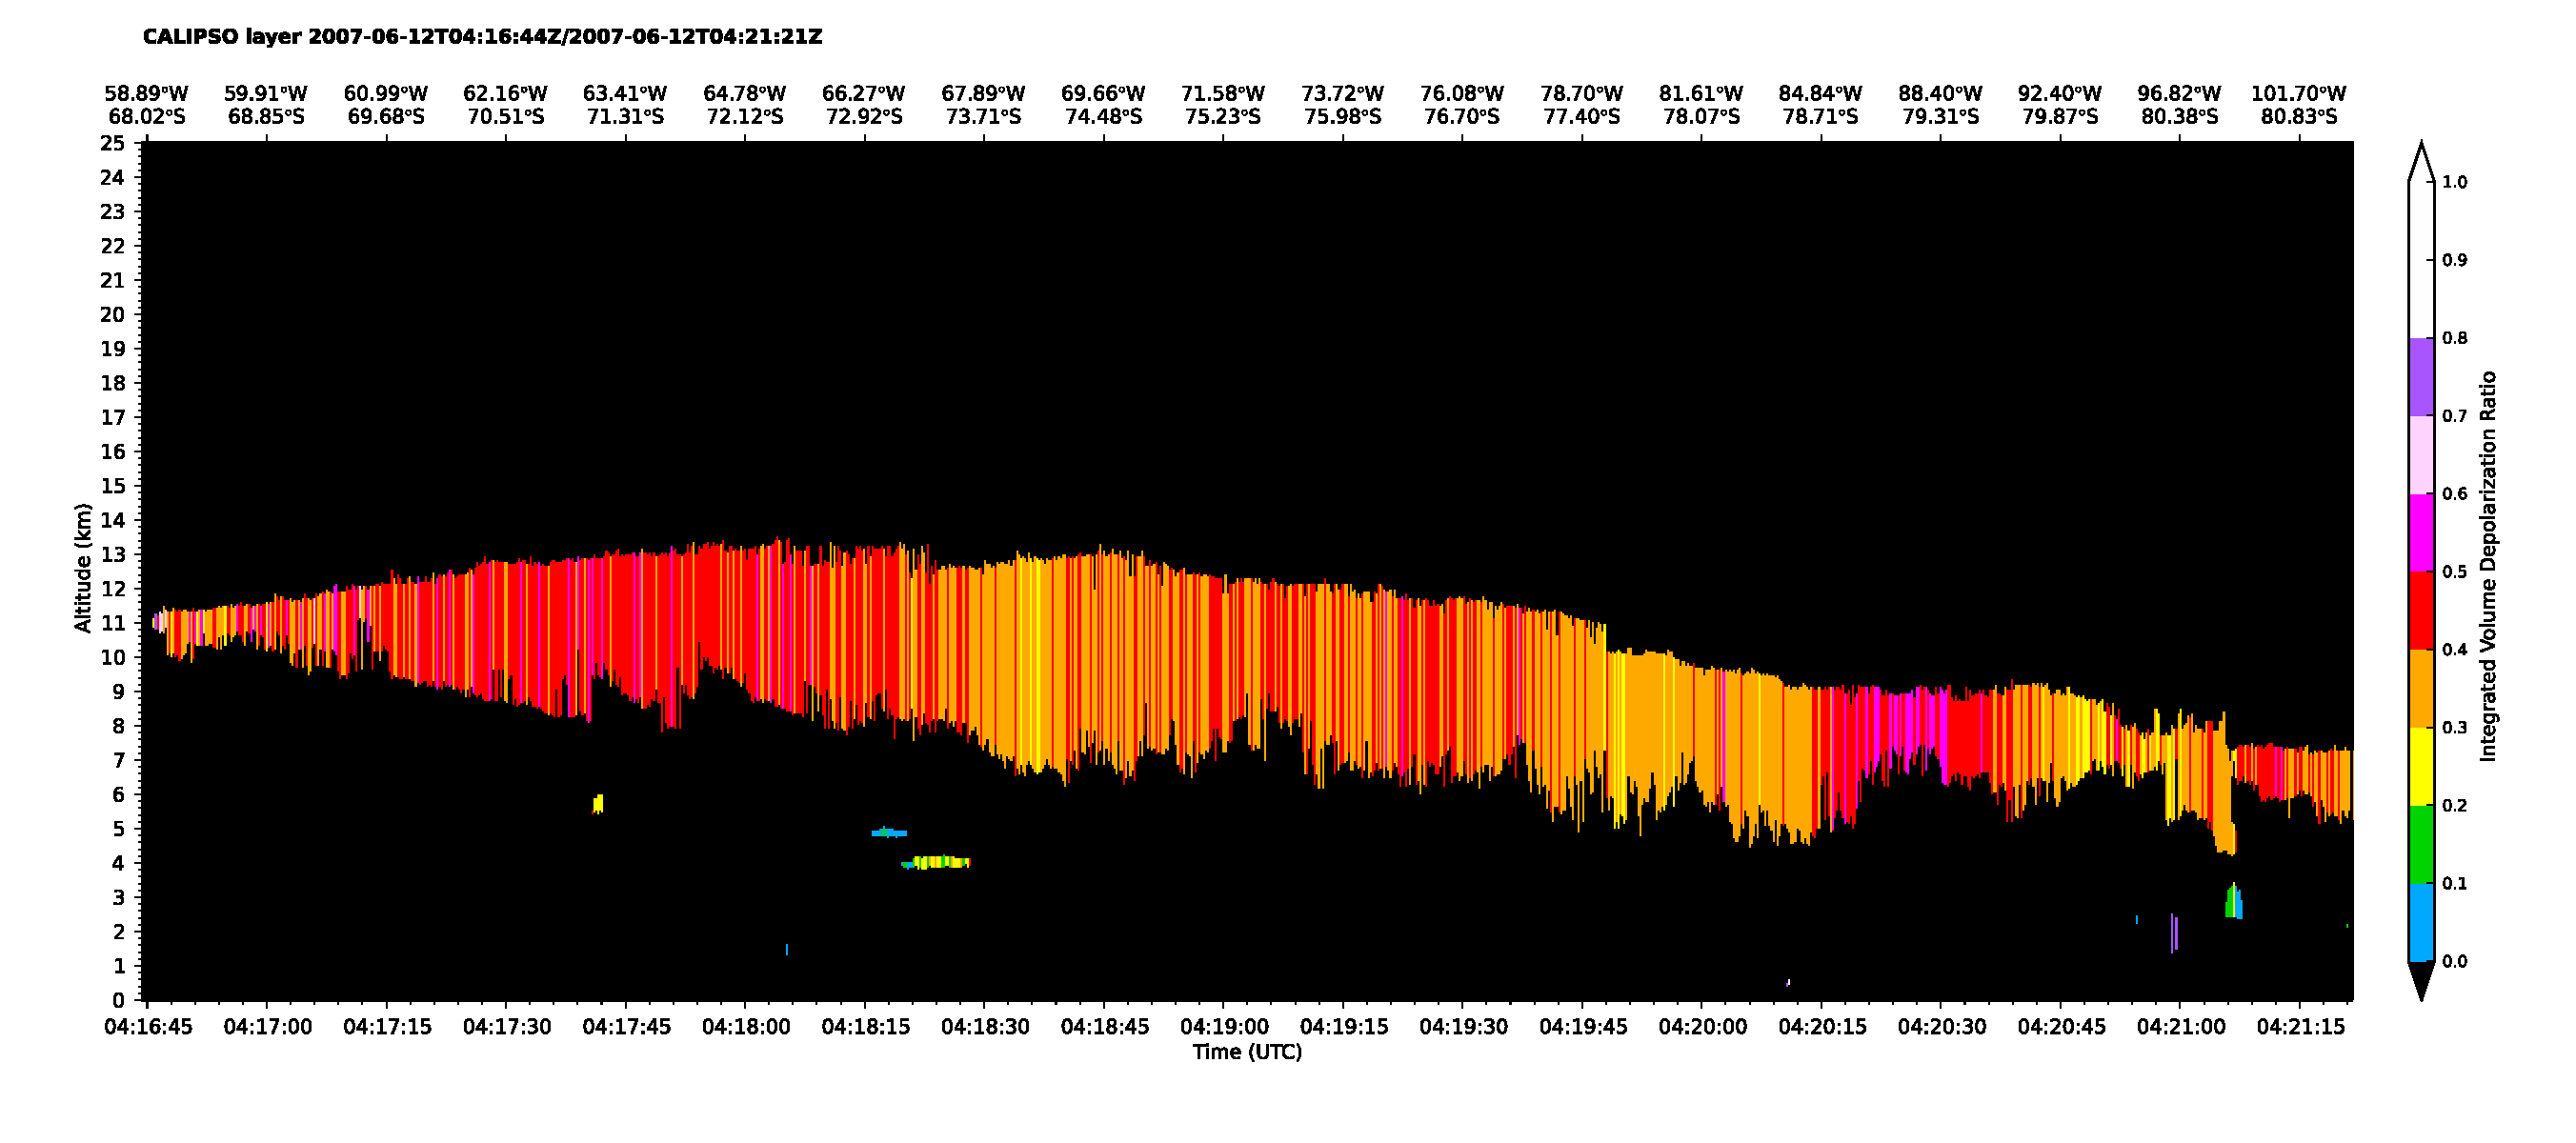
\includegraphics[width=150mm,clip,trim=10mm 10mm 4mm 4mm]{images/antarctica/1calipso-dratio-layer.pdf}\\
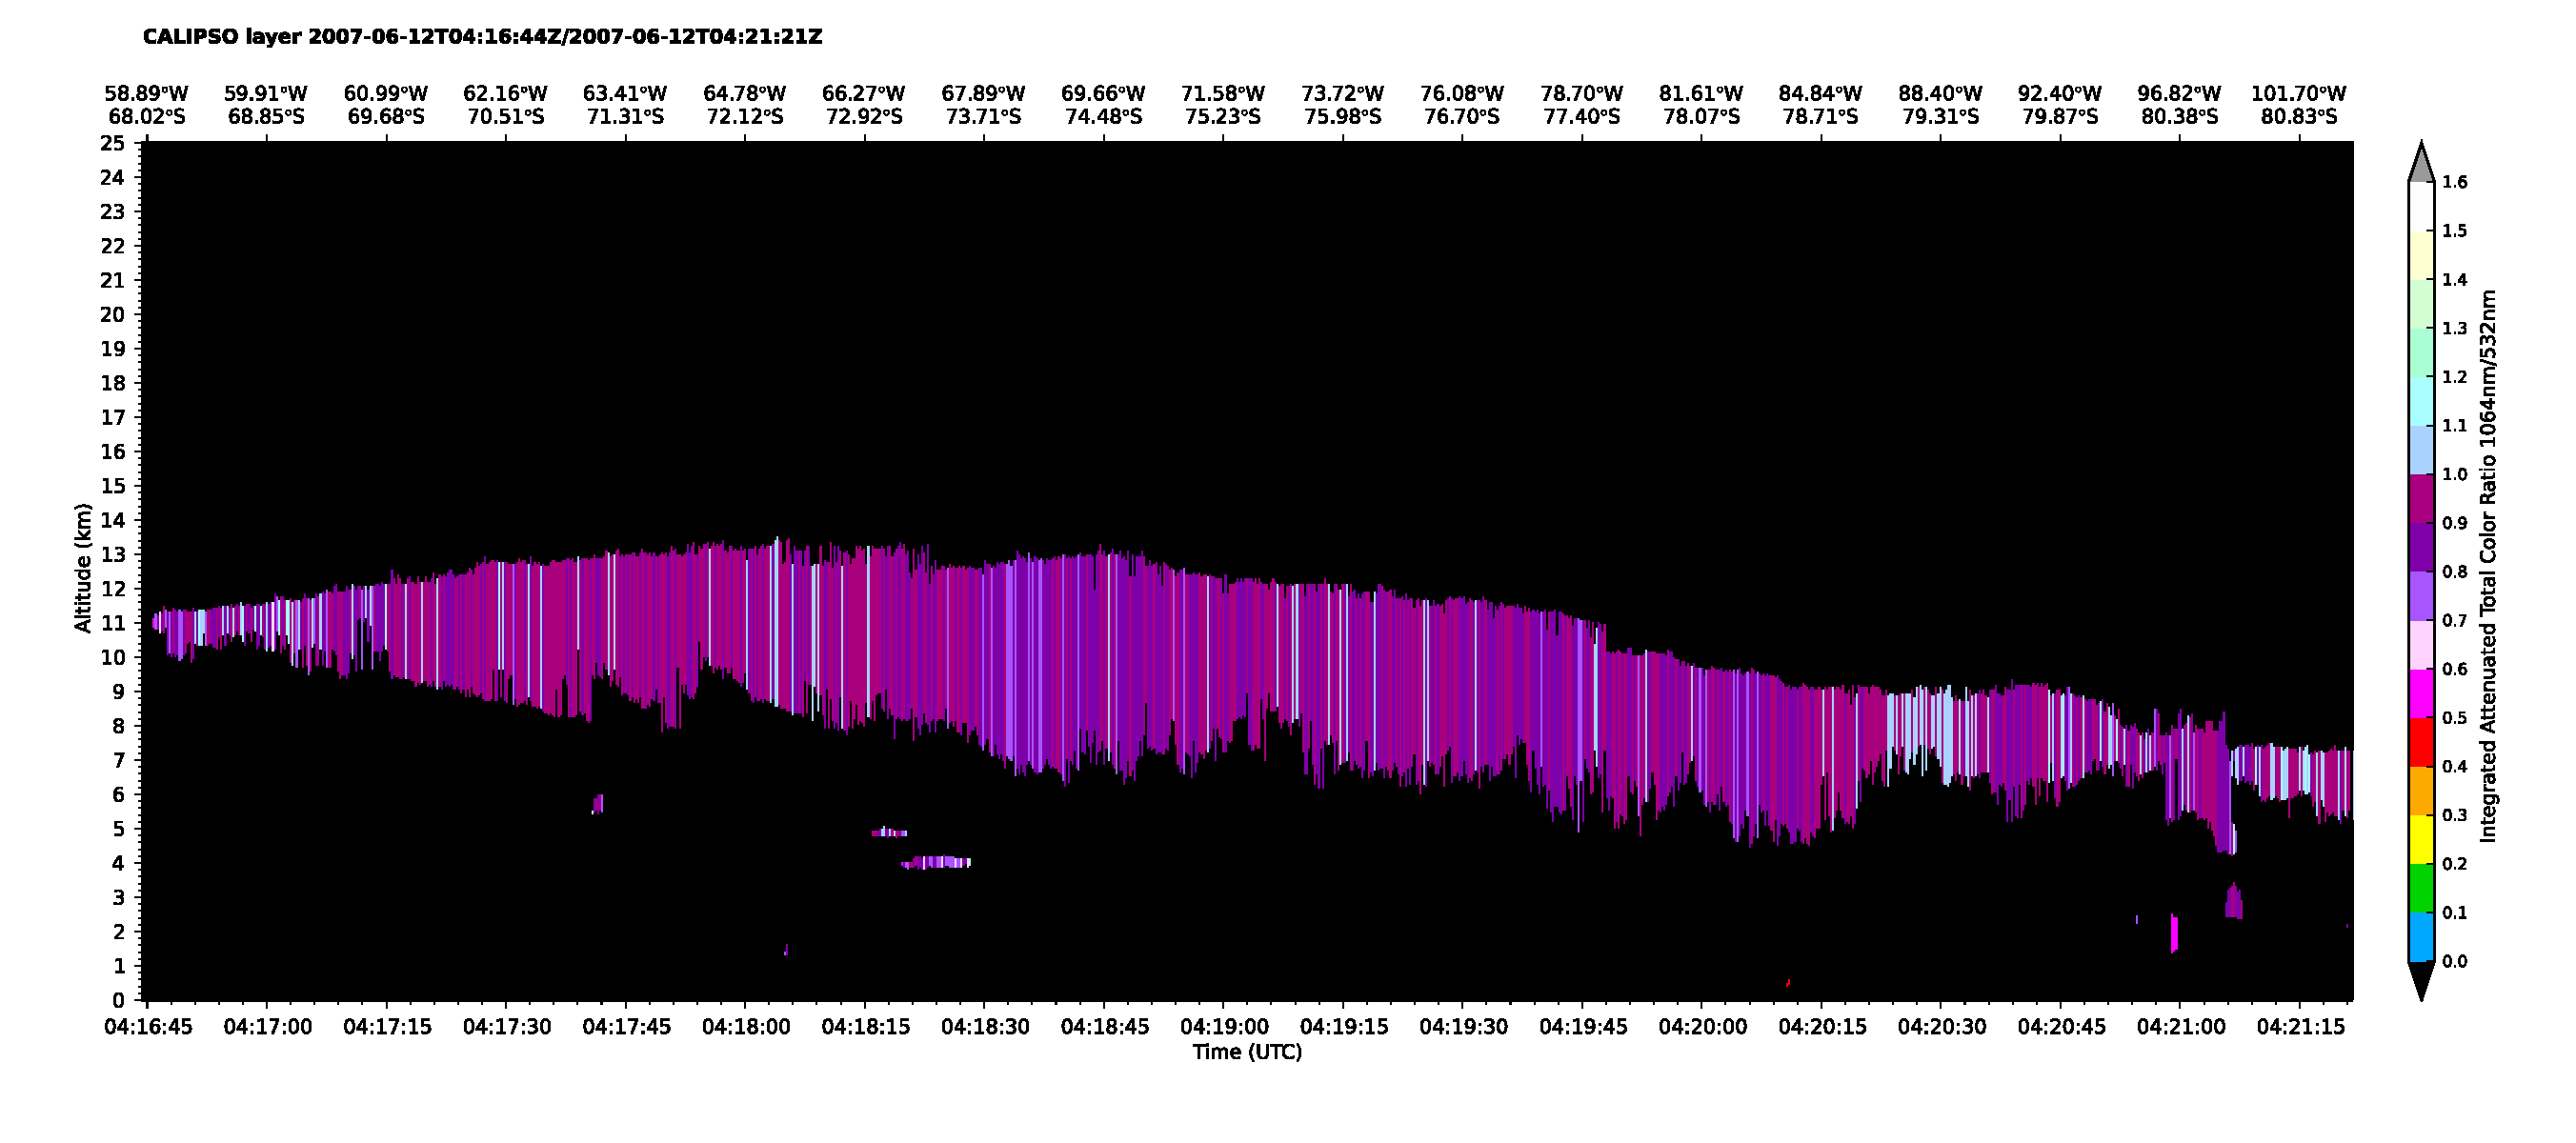
\includegraphics[width=150mm,clip,trim=10mm 10mm 4mm 4mm]{images/antarctica/1calipso-cratio-layer.pdf}

\clearpage
\noindent
\textbf{f}, the 1064-nm channel is comparable to that of \SI{532}{nm} both in
terms of strength and detected features,
but is contains more noise. \textbf{g}, the upper parts of the larger cloud were not captured by
the millimetre-wave radar, but we can see a strong response from the parts below 9 km. This suggests that
it is composed of different
particles, presumably precipitation in the form of snow pellets.
\vspace{3mm}

\noindent\textsf{e, cont.)}\\[2mm]
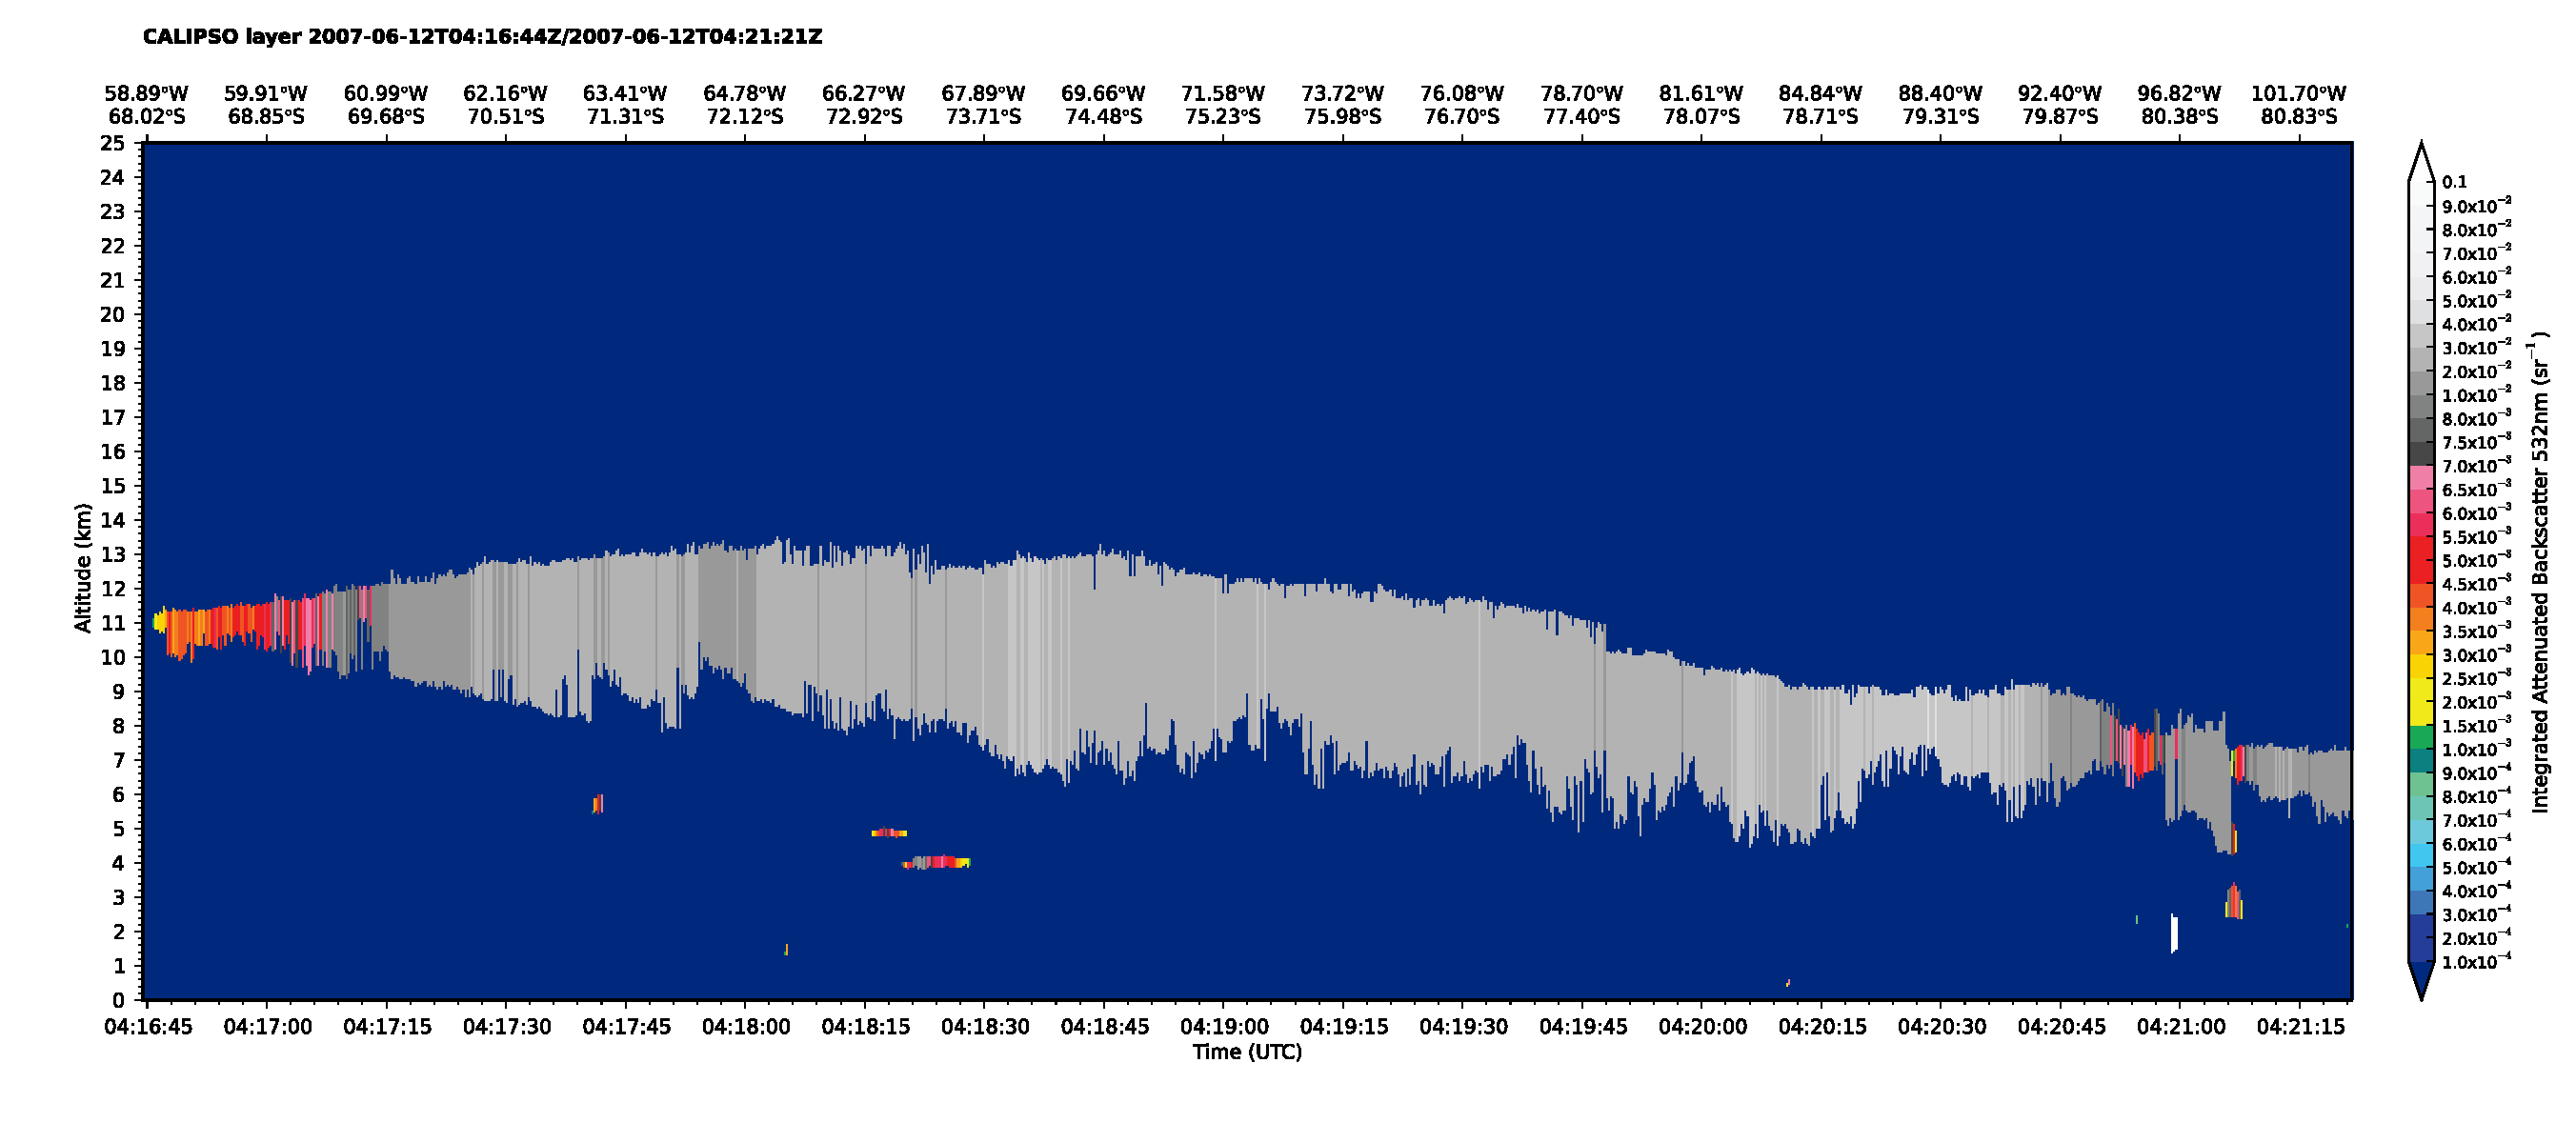
\includegraphics[width=150mm,clip,trim=10mm 10mm 4mm 4mm]{images/antarctica/1calipso532-layer.pdf}\\[-3mm]
\noindent\textsf{\small f)}\\
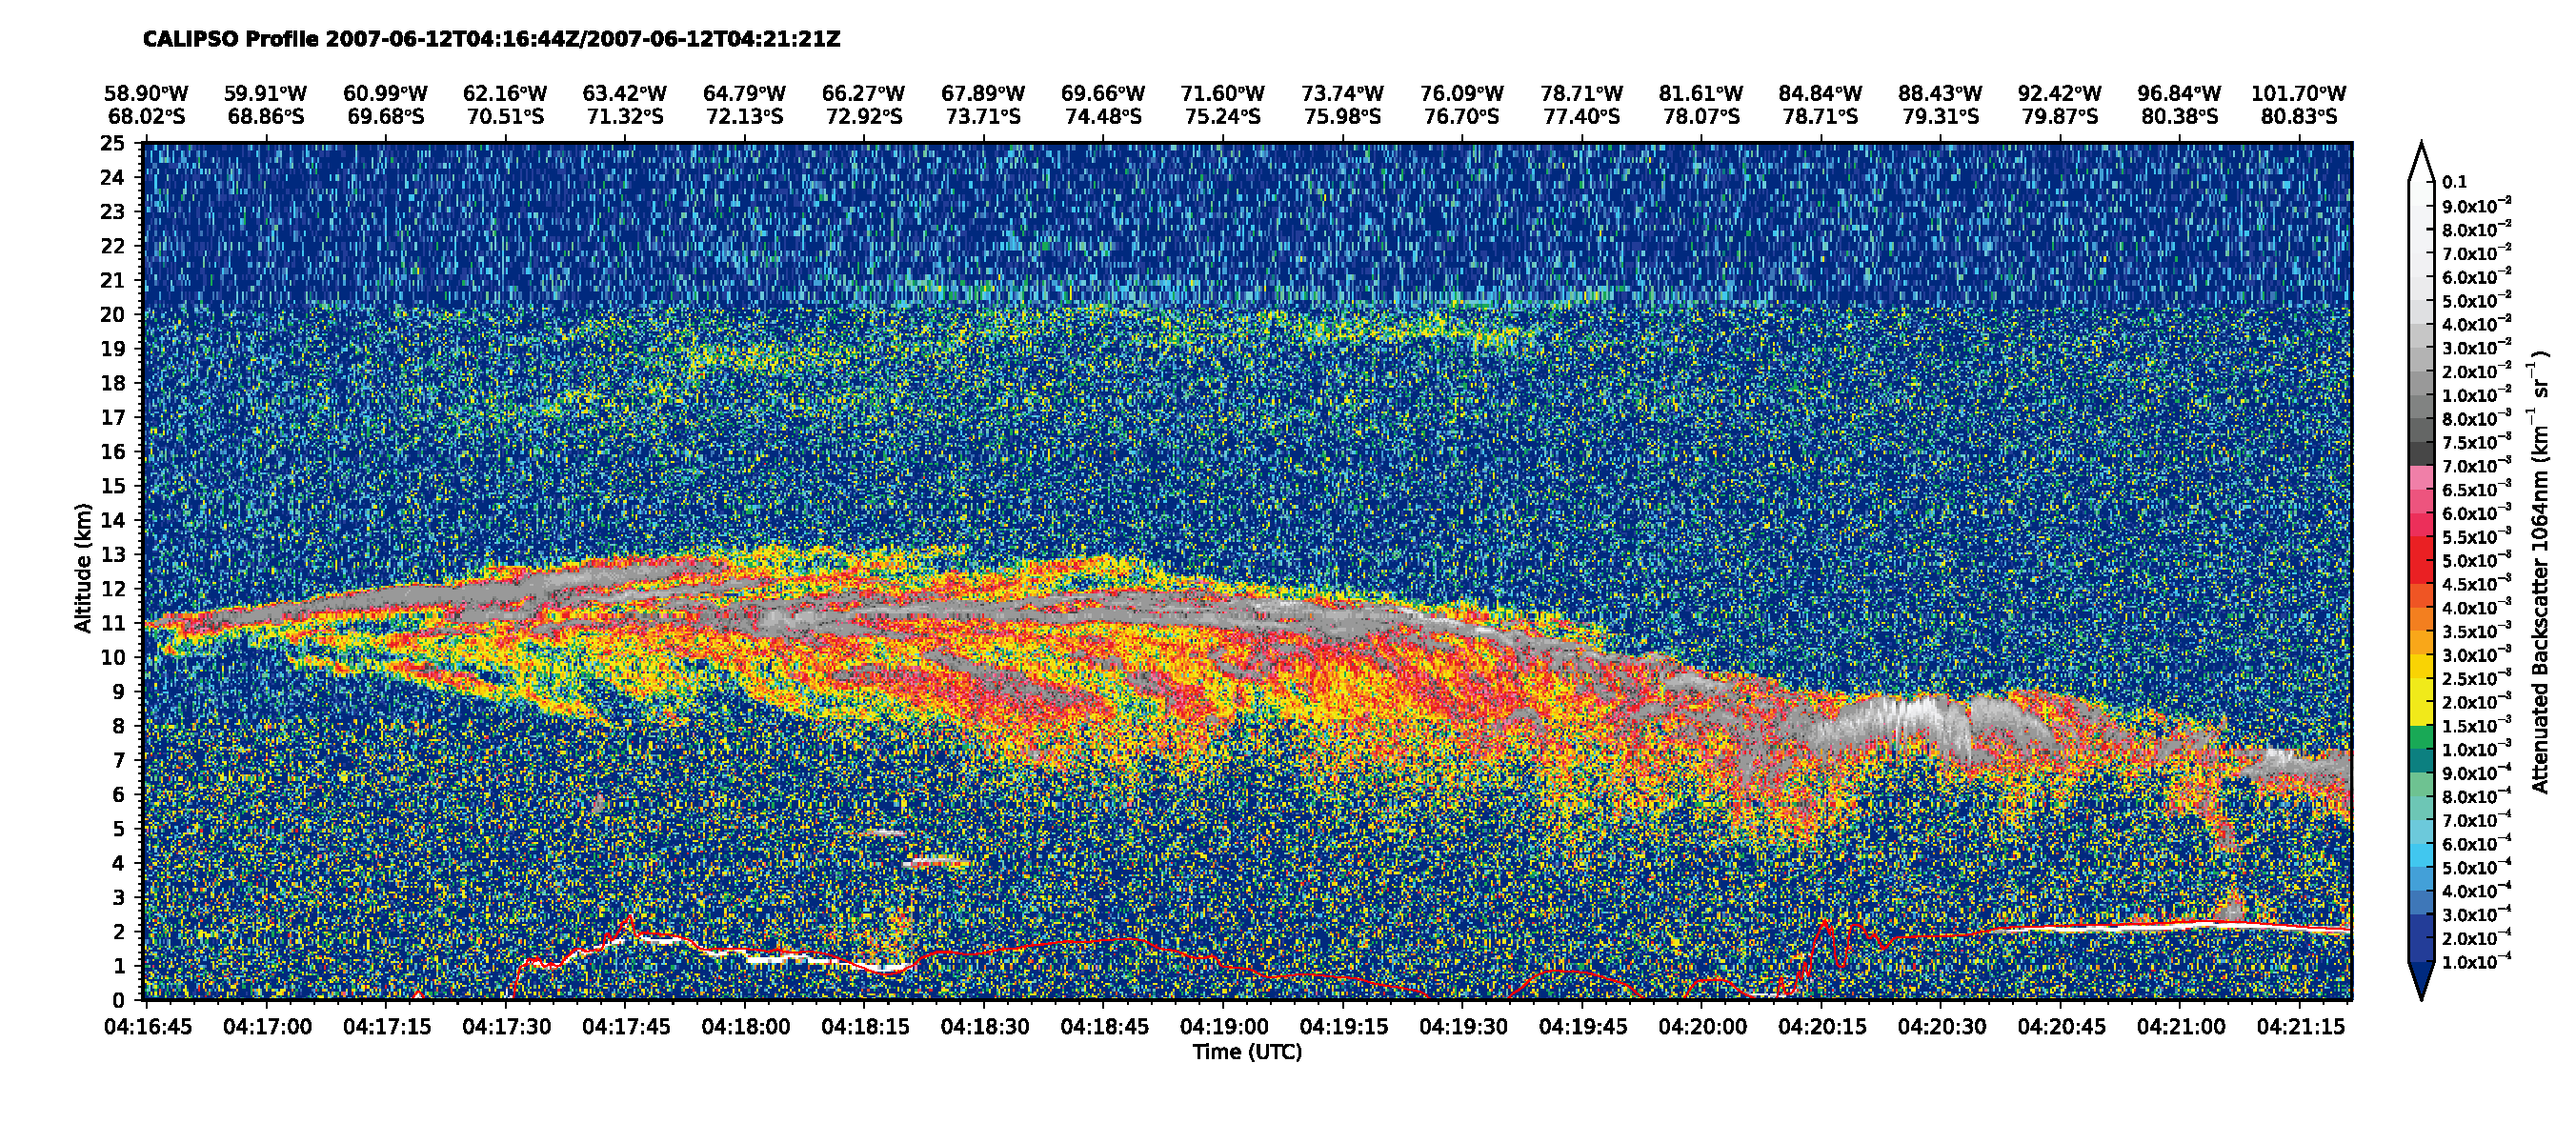
\includegraphics[width=150mm,clip,trim=10mm 10mm 4mm 4mm]{images/antarctica/1calipso1064.pdf}\\[-3mm]
\noindent\textsf{\small g)}\\
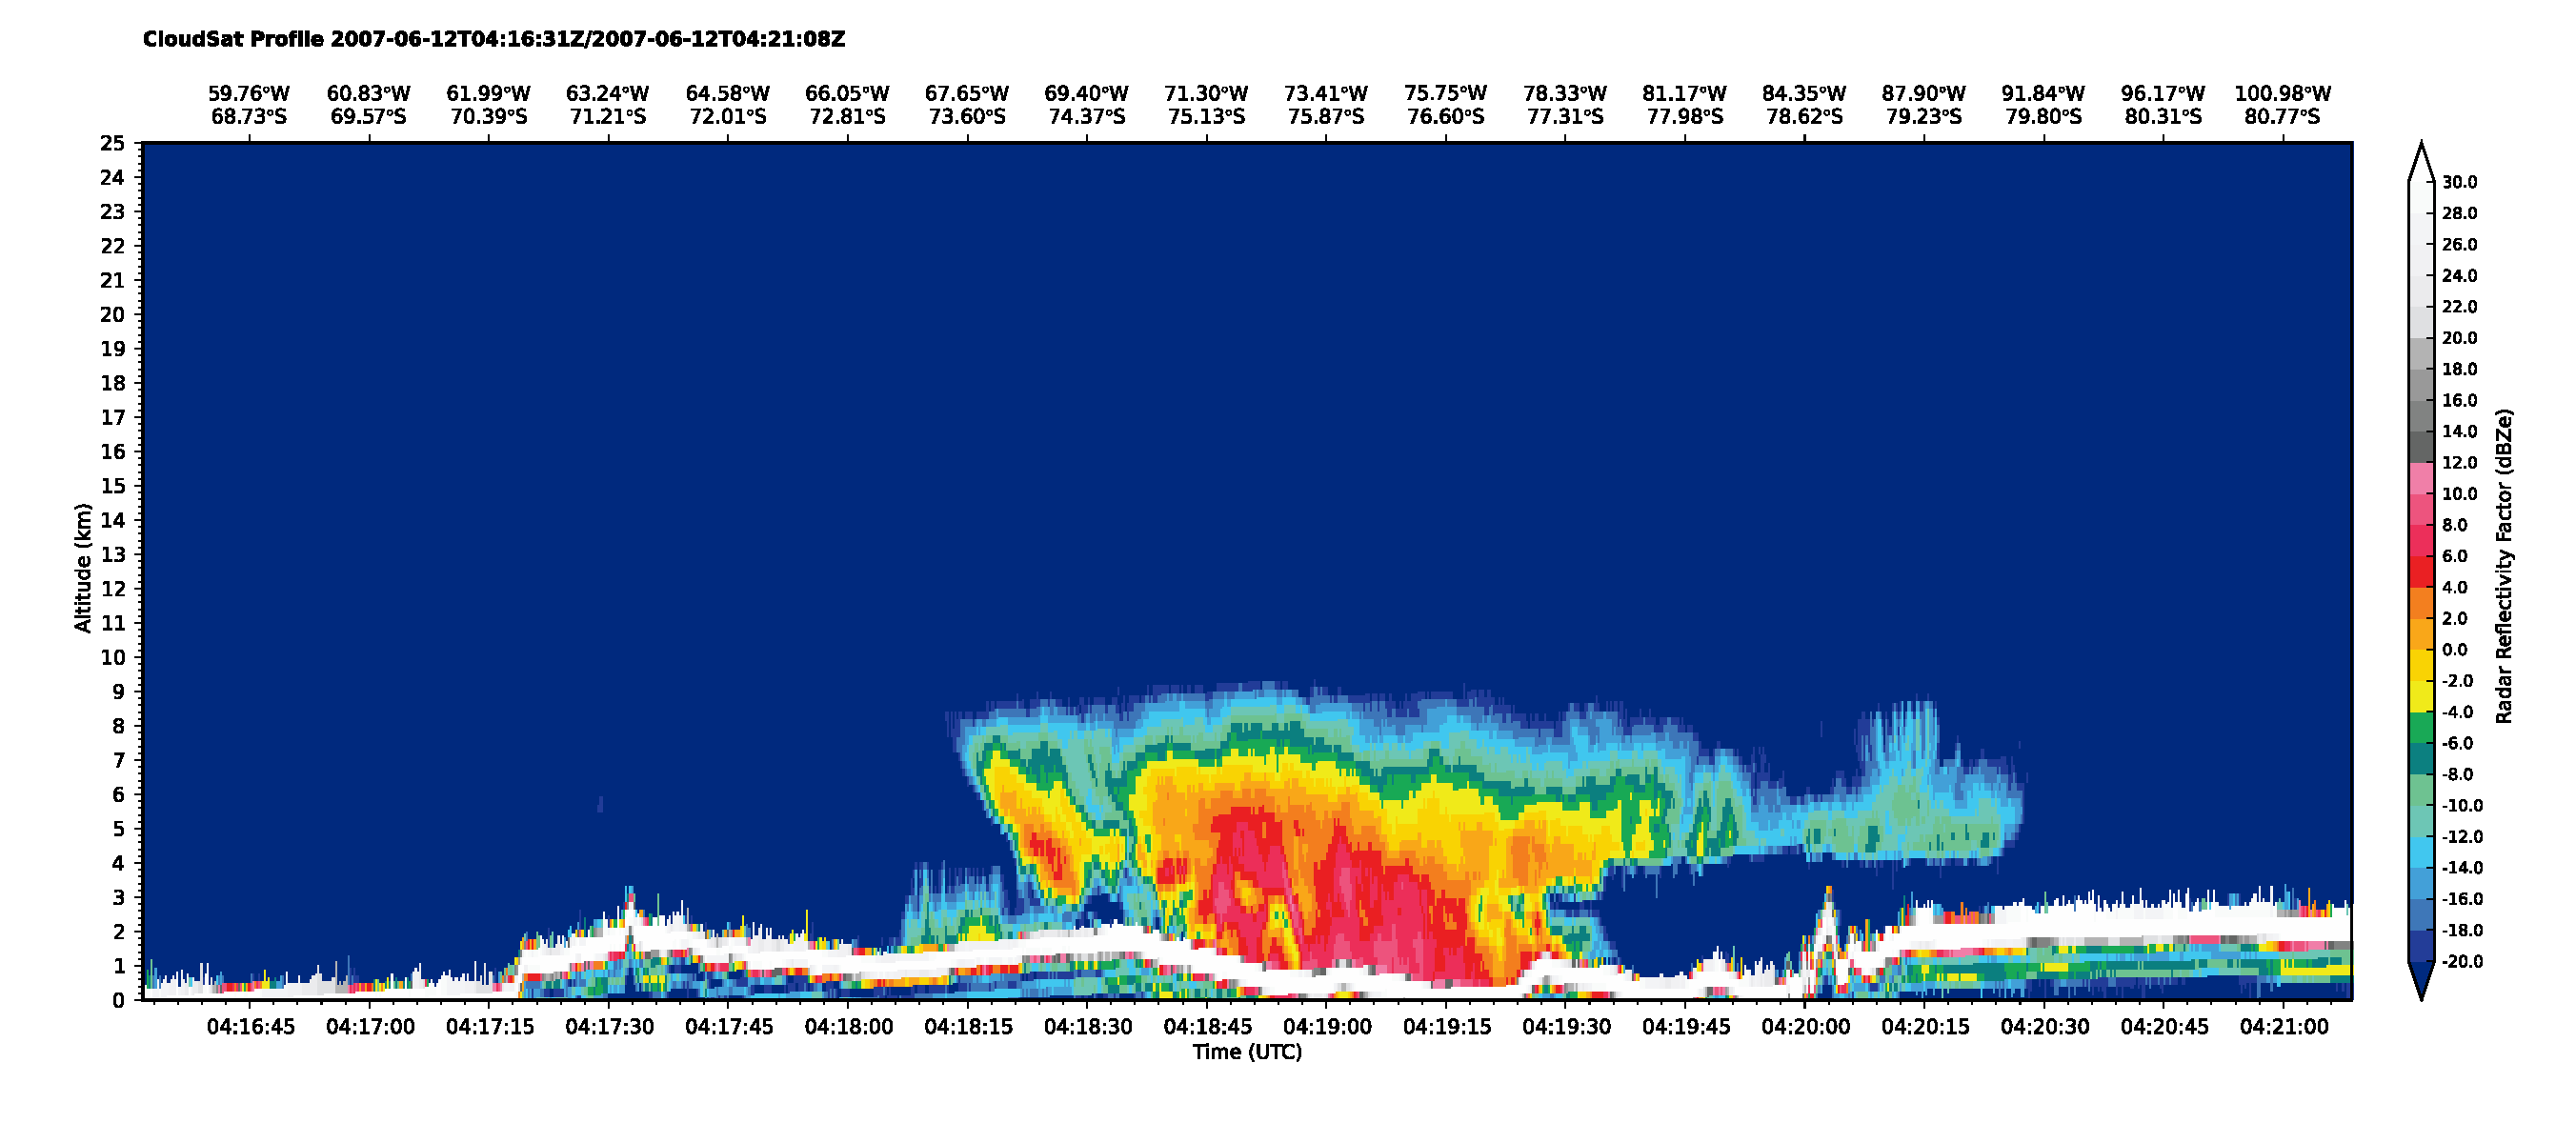
\includegraphics[width=150mm,clip,trim=10mm 10mm 4mm 4mm]{images/antarctica/1cloudsat-reflec.pdf}

\clearpage
\section*{Case 3: Overshooting Top, Mexico, 16 July 2007}
This case presents the appearance of a cumulonimbus (Cb) cloud with an overshooting top.
\vspace{3mm}

\noindent
\begin{minipage}[t]{78mm}
\textbf{a}, The Cb was located in the south of
Mexico at 3:36\,am
local time. In particular, CALIPSO flew over its overshooting top at 8:36:31~UTC,
as can be recognised on the swath by brightness temperature as low as
\SI{-80}{\celsius}. \textbf{b},
the entire cloud is best observable with CPR. Reflectivity is strongest near the
centre of the cloud, probably because it contains hail or partly melted ice
particles, which generate high response at this wavelength. \textbf{c}, in
contrast with
CPR, CALIOP only captures the anvil and the overshooting top of the Cb. This
lies at a very high altitude of about \SI{14}{km}. Response is extremely strong
from
the overshooting top (more than \SI{0.1}{km^{-1} sr^{-1}}). 
\end{minipage}\hfill
\begin{minipage}[t]{68mm}
\noindent\textsf{\small a)}\\
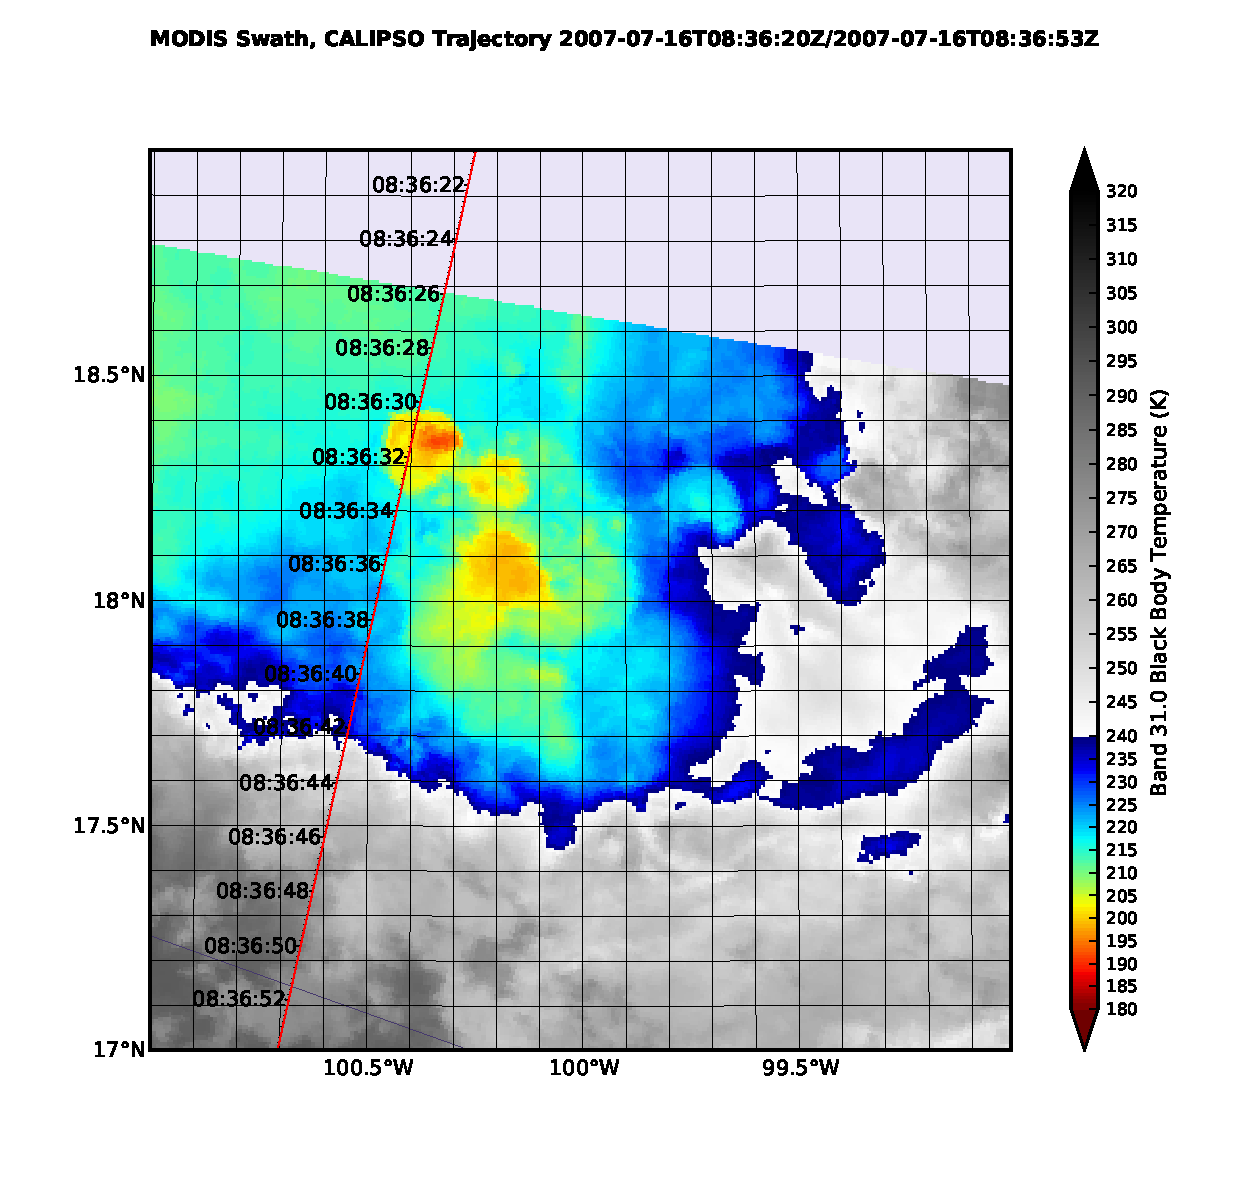
\includegraphics[width=68mm,clip,trim=10mm 10mm 4mm 4mm]{images/overshooting-top/orbit-modis_x31+calipso.pdf}\\
\end{minipage}
\vspace{5mm}

\noindent\textsf{\small b)}\\
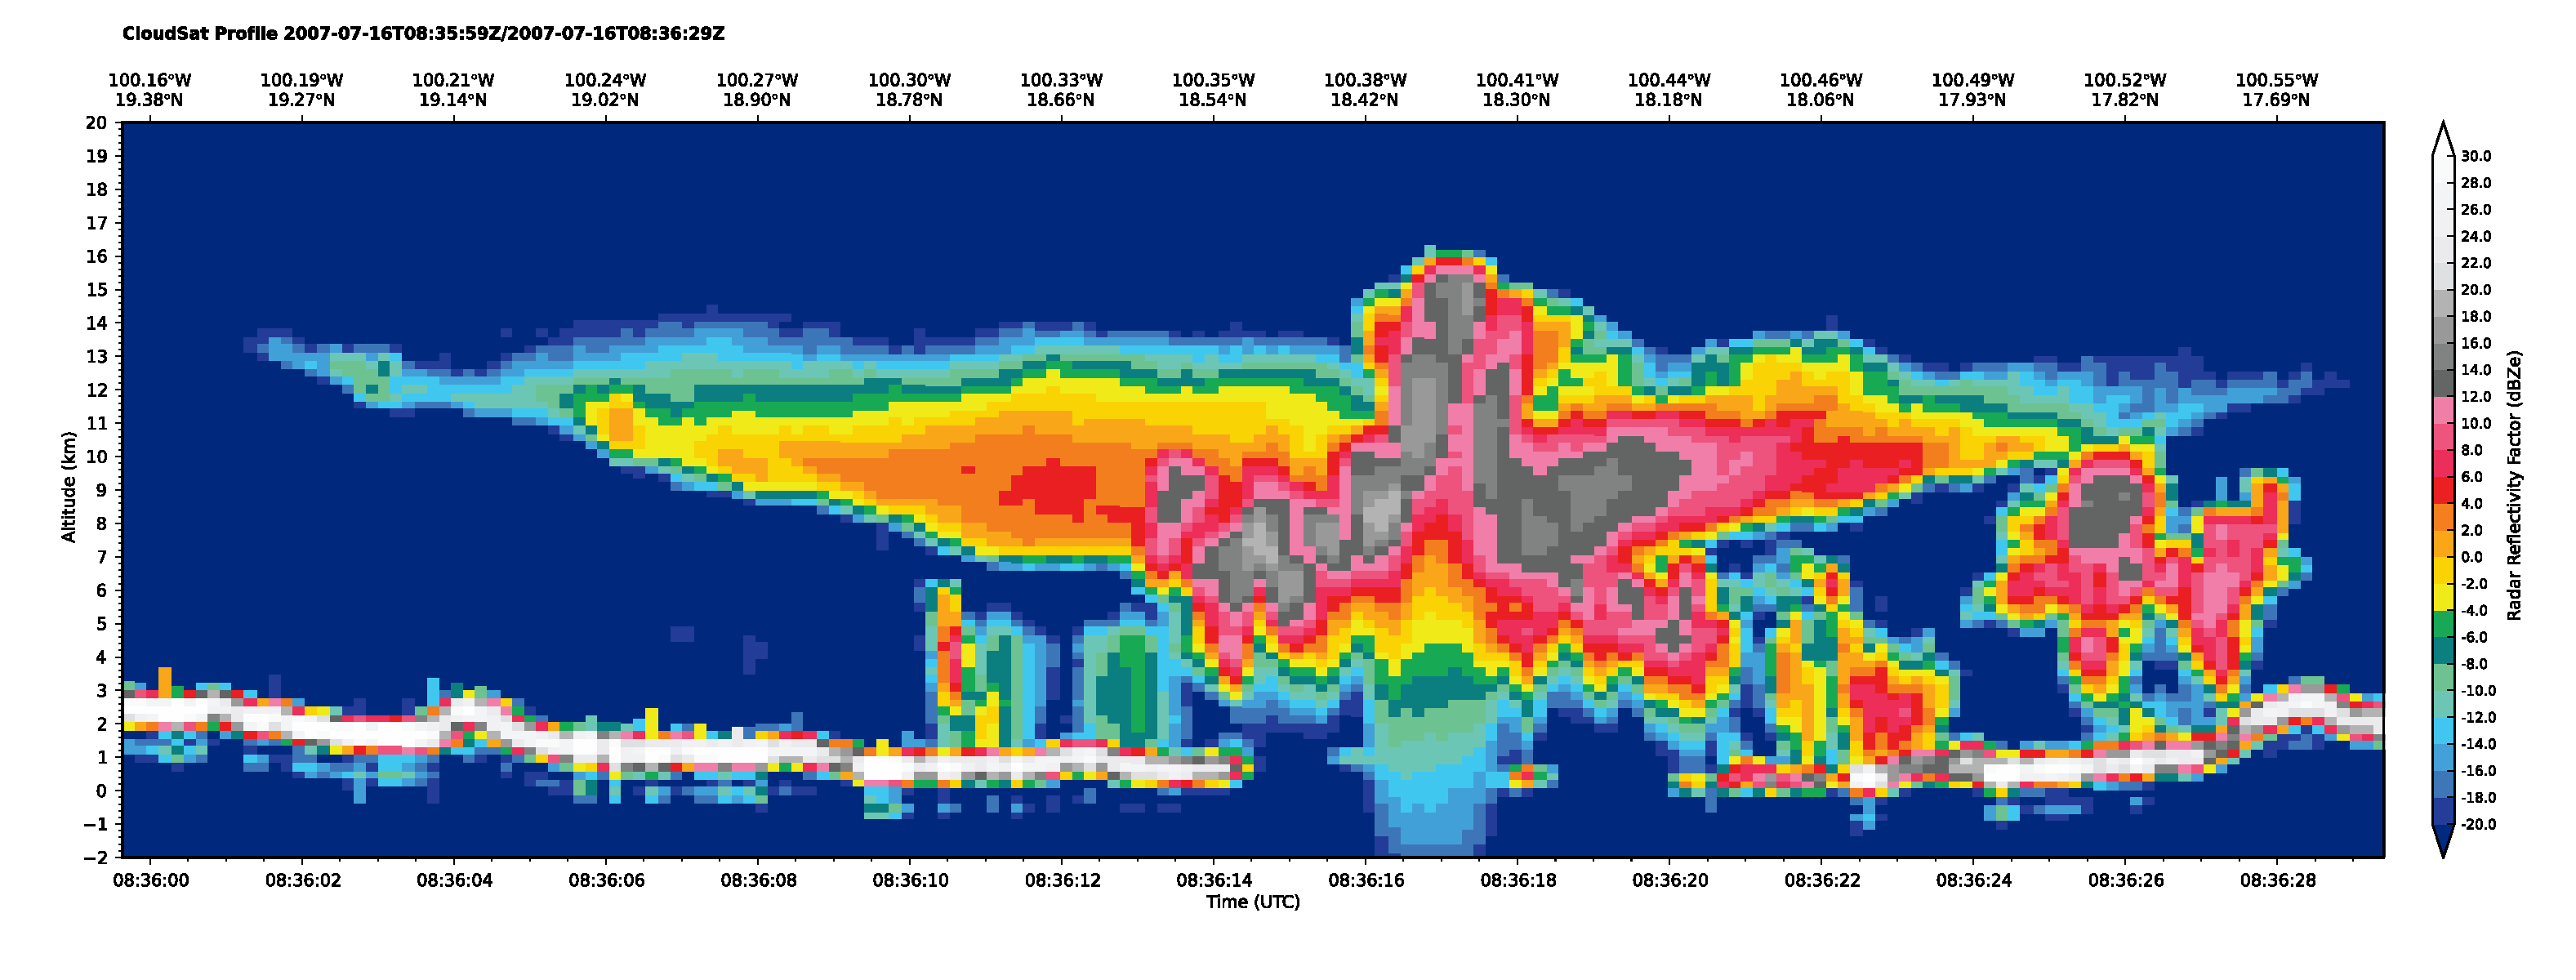
\includegraphics[width=150mm,clip,trim=10mm 10mm 4mm 4mm]{images/overshooting-top/1cloudsat-reflec.pdf}\\
\noindent\textsf{\small c)}\\
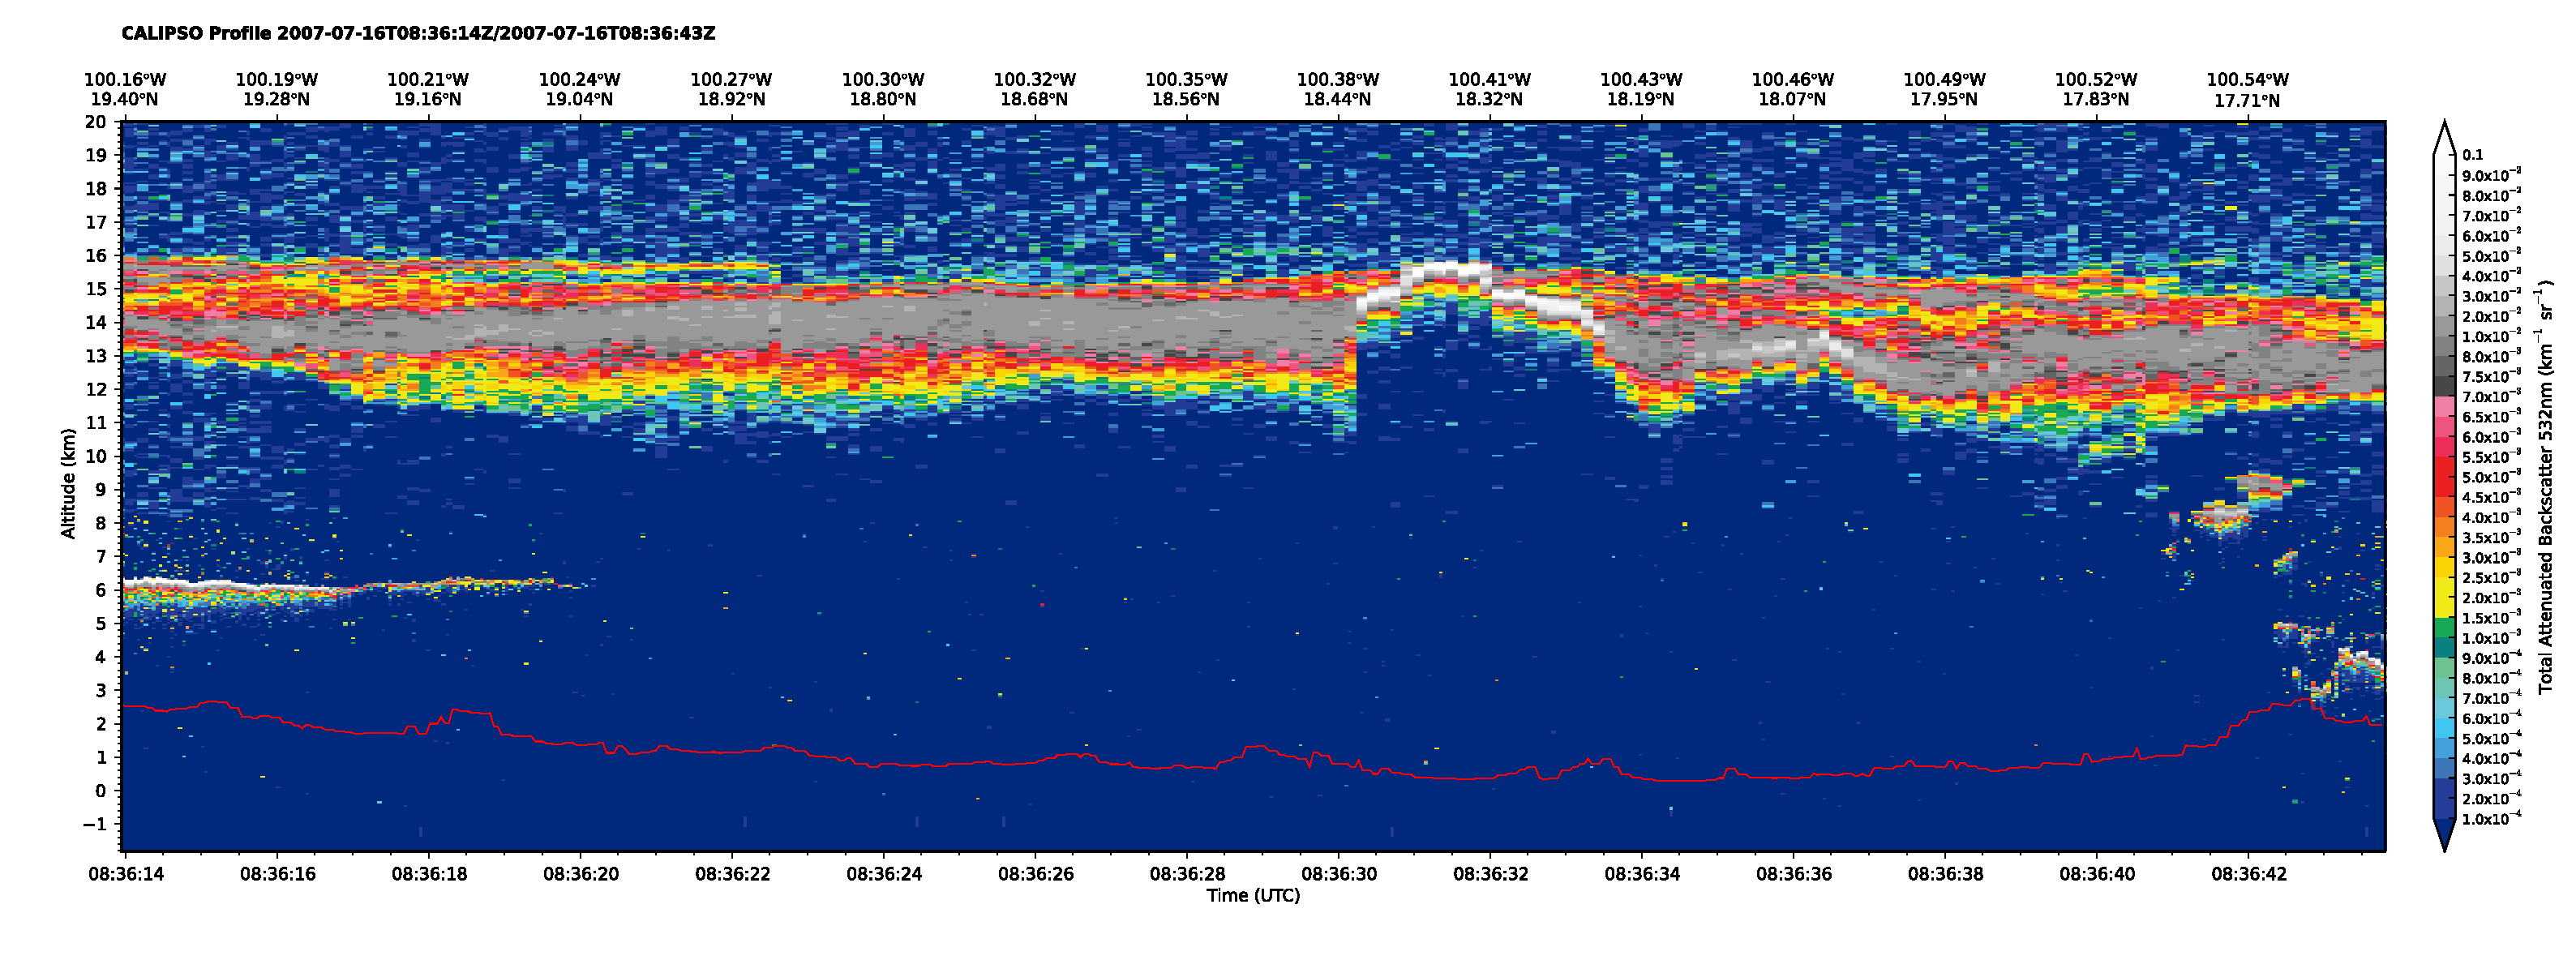
\includegraphics[width=150mm,clip,trim=10mm 10mm 4mm 4mm]{images/overshooting-top/1calipso532.pdf}

\clearpage
\noindent\textbf{d}, the overshooting top is much colder than the anvil, \textbf{e}, and polarises light more strongly.
\vspace{3mm}

\noindent\textsf{\small d)}\\
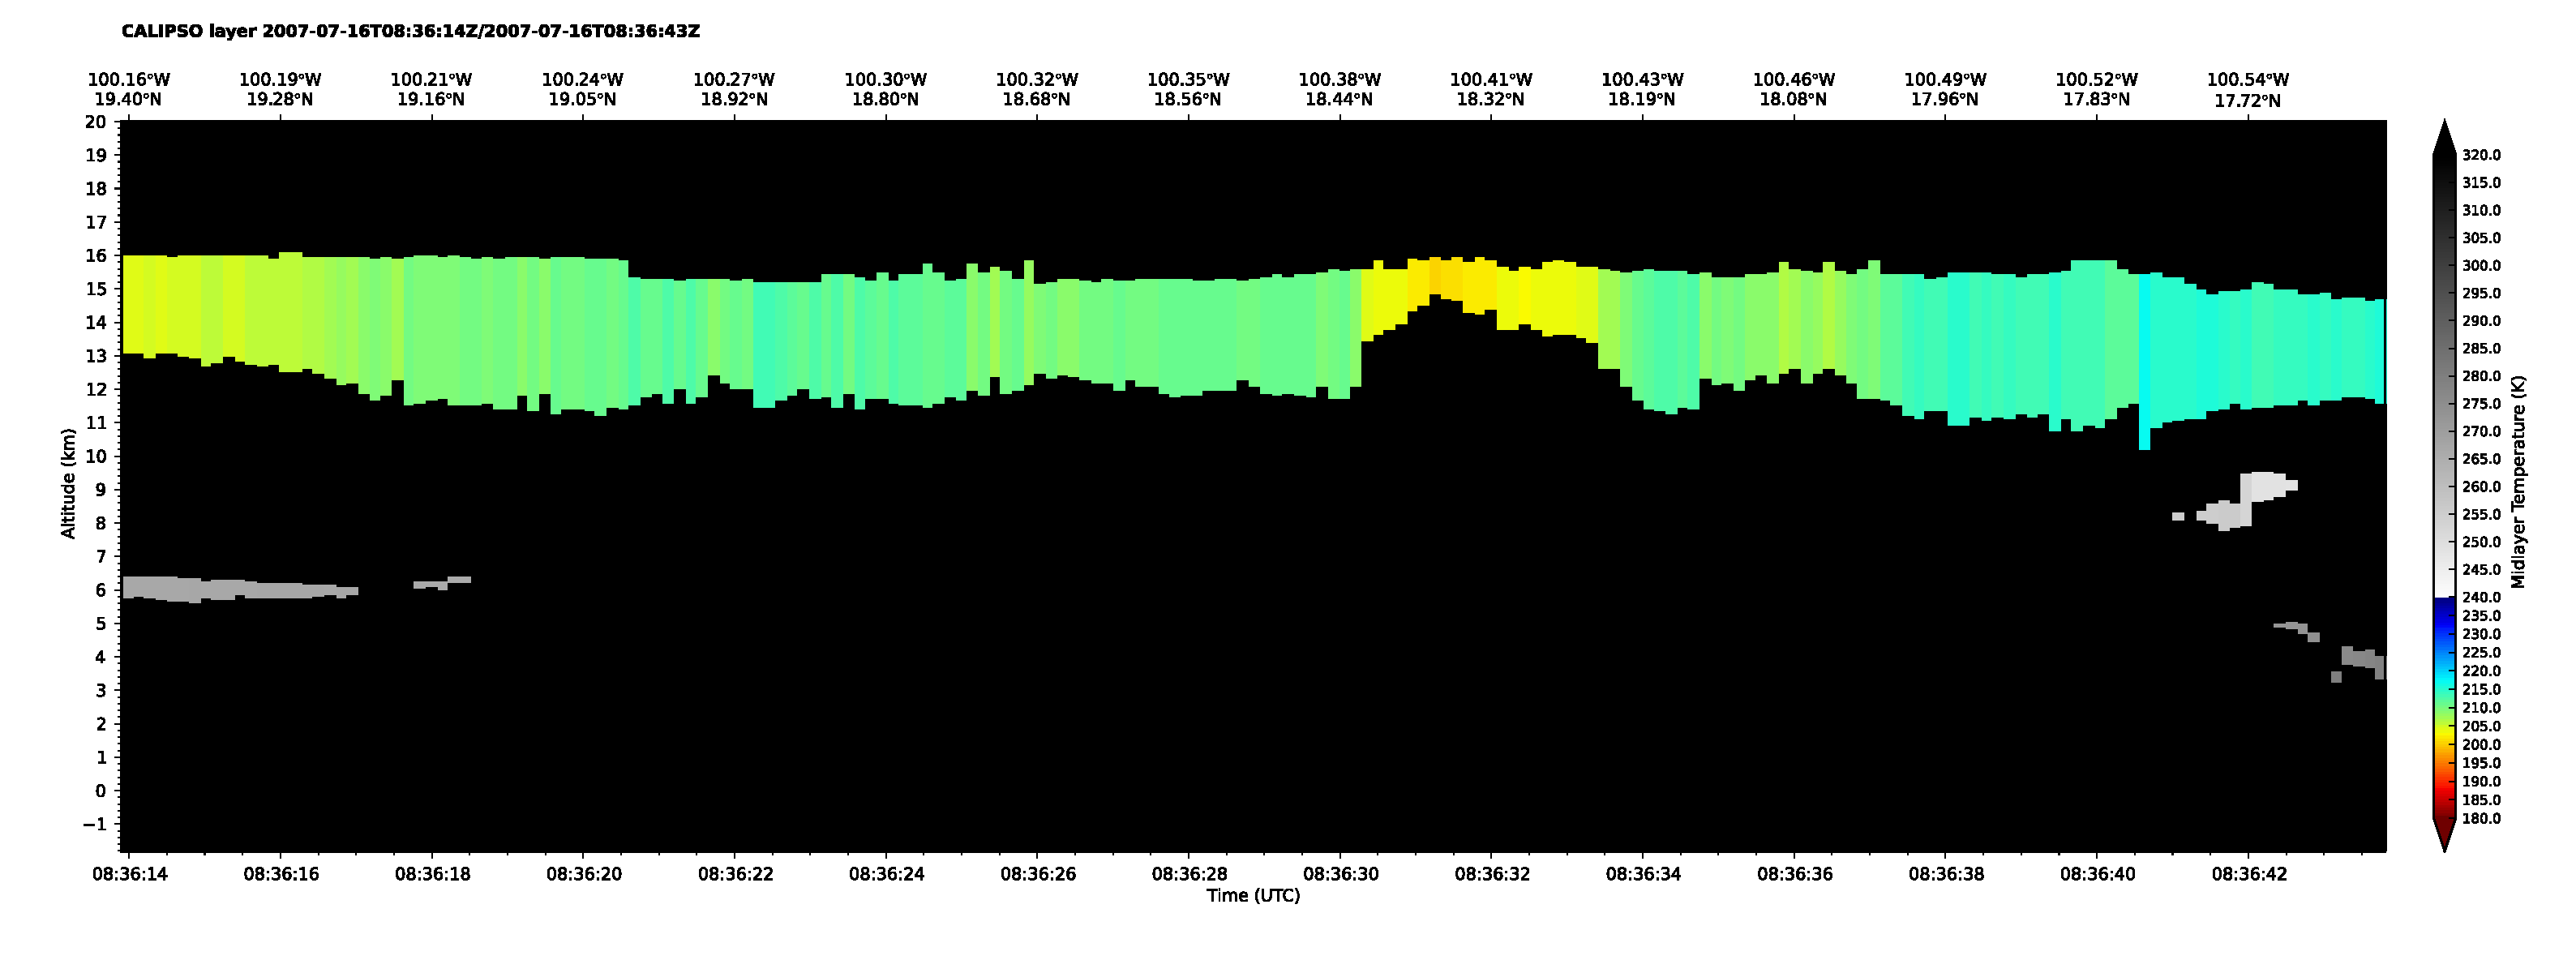
\includegraphics[width=150mm,clip,trim=10mm 10mm 4mm 4mm]{images/overshooting-top/1calipso-temperature-layer.pdf}\\
\noindent\textsf{\small e)}\\
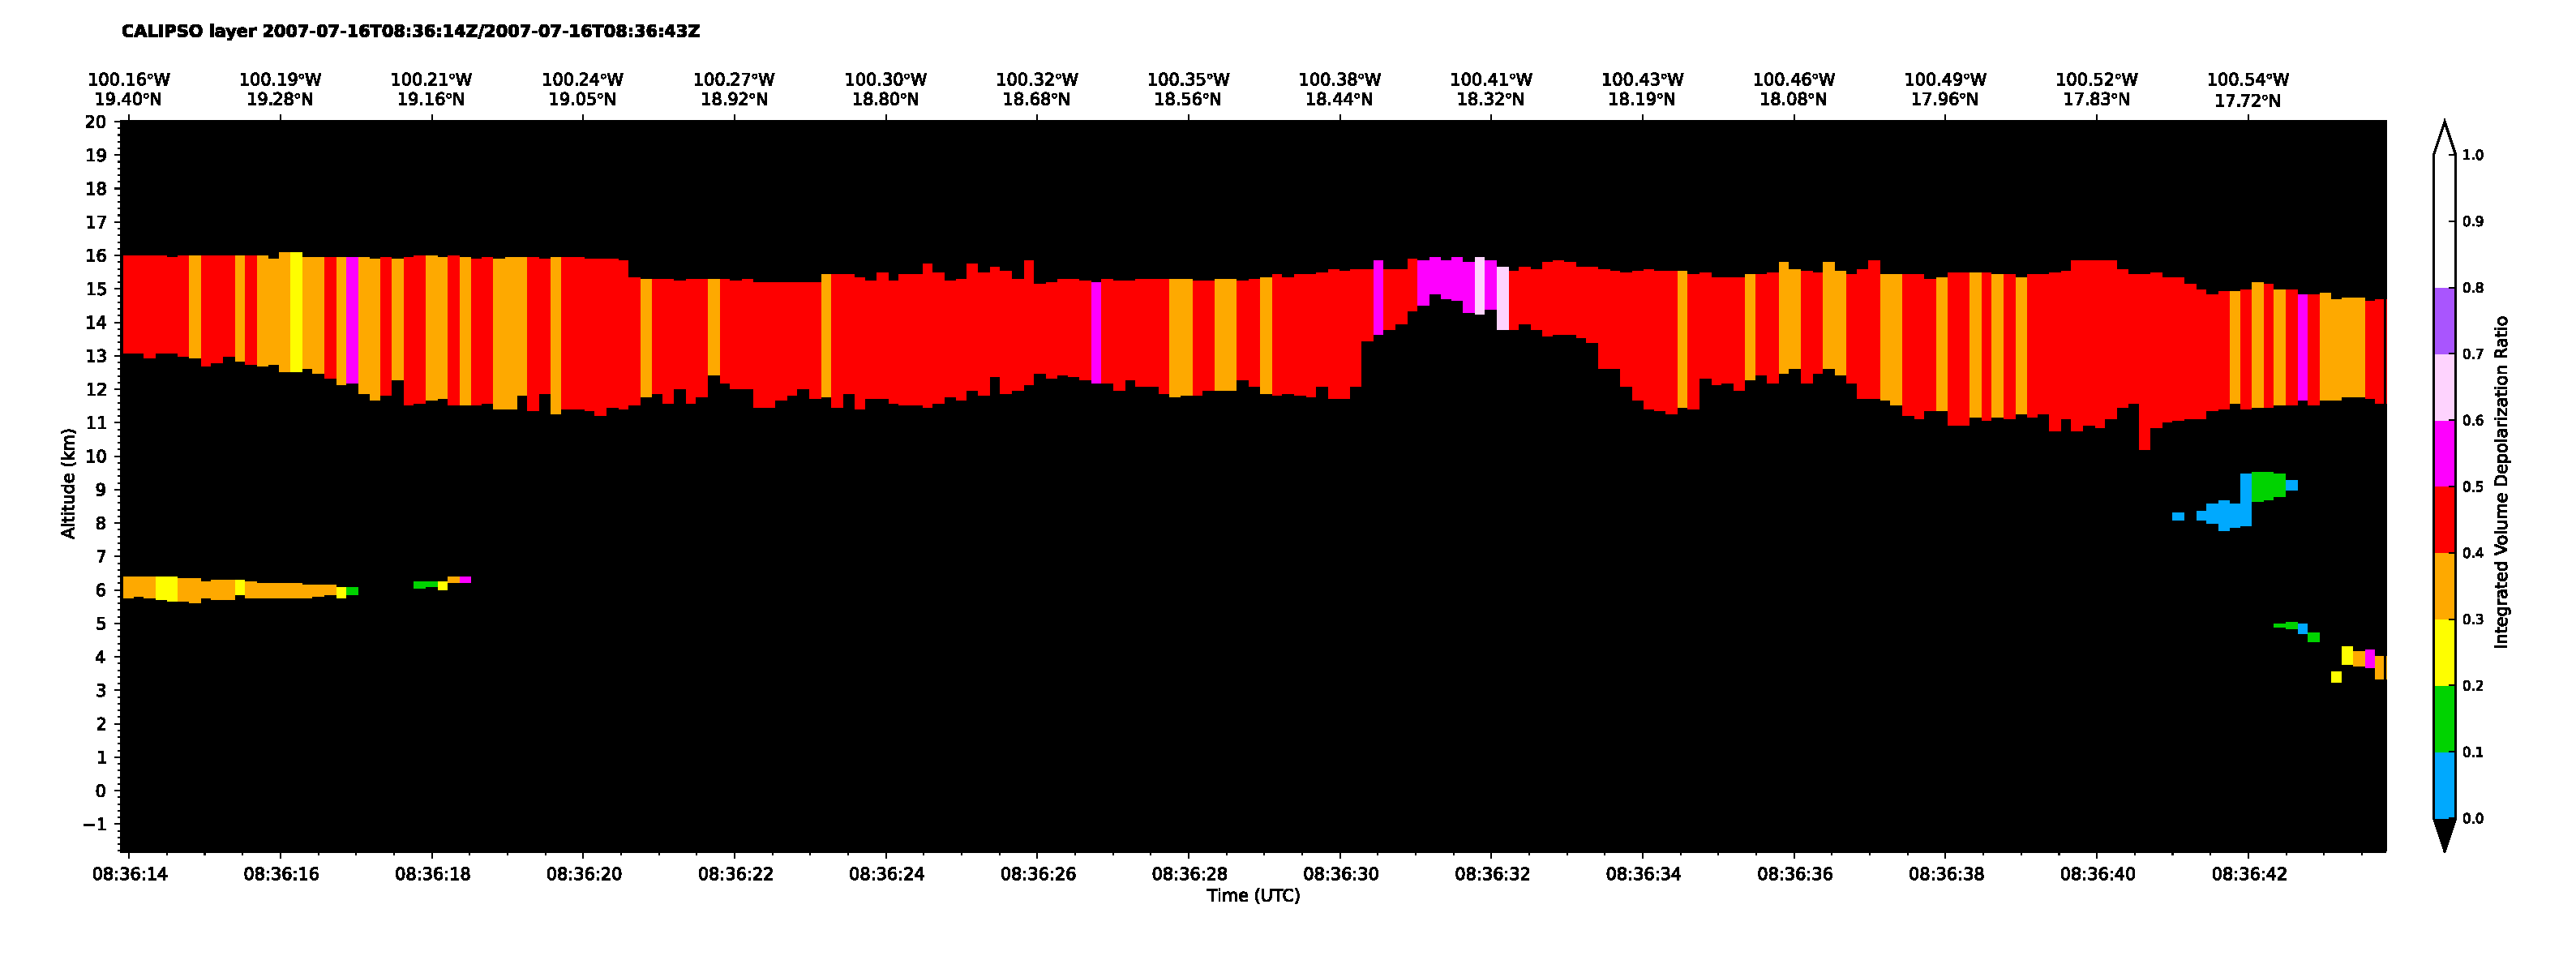
\includegraphics[width=150mm,clip,trim=10mm 10mm 4mm 4mm]{images/overshooting-top/1calipso-dratio-layer.pdf}\\

\normalsize\rmfamily